\documentclass[chi_draft]{sigchi}

% Use this section to set the ACM copyright statement (e.g. for
% preprints).  Consult the conference website for the camera-ready
% copyright statement.

% Copyright
\CopyrightYear{2018}
%\setcopyright{acmcopyright}
\setcopyright{acmlicensed}
%\setcopyright{rightsretained}
%\setcopyright{usgov}
%\setcopyright{usgovmixed}
%\setcopyright{cagov}
%\setcopyright{cagovmixed}
% DOI
\doi{http://dx.doi.org/10.475/123_4}
% ISBN
\isbn{123-4567-24-567/08/06}
%Conference
\conferenceinfo{CHI'16,}{May 07--12, 2016, San Jose, CA, USA}
%Price
\acmPrice{\$15.00}

% Use this command to override the default ACM copyright statement
% (e.g. for preprints).  Consult the conference website for the
% camera-ready copyright statement.

%% HOW TO OVERRIDE THE DEFAULT COPYRIGHT STRIP --
%% Please note you need to make sure the copy for your specific
%% license is used here!
% \toappear{
% Permission to make digital or hard copies of all or part of this work
% for personal or classroom use is granted without fee provided that
% copies are not made or distributed for profit or commercial advantage
% and that copies bear this notice and the full citation on the first
% page. Copyrights for components of this work owned by others than ACM
% must be honored. Abstracting with credit is permitted. To copy
% otherwise, or republish, to post on servers or to redistribute to
% lists, requires prior specific permission and/or a fee. Request
% permissions from \href{mailto:Permissions@acm.org}{Permissions@acm.org}. \\
% \emph{CHI '16},  May 07--12, 2016, San Jose, CA, USA \\
% ACM xxx-x-xxxx-xxxx-x/xx/xx\ldots \$15.00 \\
% DOI: \url{http://dx.doi.org/xx.xxxx/xxxxxxx.xxxxxxx}
% }

% Arabic page numbers for submission.  Remove this line to eliminate
% page numbers for the camera ready copy
% \pagenumbering{arabic}

% Load basic packages
\usepackage{balance}       % to better equalize the last page
\usepackage{graphics}      % for EPS, load graphicx instead 
\usepackage[T1]{fontenc}   % for umlauts and other diaeresis
\usepackage{txfonts}
\usepackage{mathptmx}
\usepackage[pdflang={en-US},pdftex]{hyperref}
\usepackage{color}
\usepackage{booktabs}
\usepackage{textcomp}

% Some optional stuff you might like/need.
\usepackage{microtype}        % Improved Tracking and Kerning
% \usepackage[all]{hypcap}    % Fixes bug in hyperref caption linking
\usepackage{ccicons}          % Cite your images correctly!
% \usepackage[utf8]{inputenc} % for a UTF8 editor only

% If you want to use todo notes, marginpars etc. during creation of
% your draft document, you have to enable the "chi_draft" option for
% the document class. To do this, change the very first line to:
% "\documentclass[chi_draft]{sigchi}". You can then place todo notes
% by using the "\todo{...}"  command. Make sure to disable the draft
% option again before submitting your final document.
\usepackage{todonotes}

% Paper metadata (use plain text, for PDF inclusion and later
% re-using, if desired).  Use \emtpyauthor when submitting for review
% so you remain anonymous.


\def\plaintitle{As We May Study: Towards the Web as a Personalized Language Textbook}
% As We May Study: The Web as a Personalized Language Textbook
% News and Blogs as the Source of Material for the Language Textbooks of the Future
% As We May Study: The Potential of the The Web as the Language Textbook of the Future
% As We May Study: Perspectives on the The Web as the Language Textbook of the Future
% As We May Study: Highschool Students Meet the Language Textbook of the Future
% instead of meet: face / encounter
% The Language Learning of the Future: Personal, Interesting, Adaptive
% Enabling Personalized Free Reading for Second Language Acquisition
% The Textbook of the Present: Personal, Adaptable, Interesting
% The Textbook for the Generation Y: Contextual, Personal, Adaptable
% The Language Learning of the Present: Personal, Interesting, Adaptive
% An Adaptive Reading Platform for Accelerating Vocabulary Acquisition: Because Good Enough for Everybody is Exciting for Nobody: Why Should We 
% The Myth of the Average Language Reader in 
% Highschool Students Meet the Language Textbook of the Future


\def\plainauthor{First Author, Second Author, Third Author,
  Fourth Author, Fifth Author, Sixth Author}
\def\emptyauthor{}
\def\plainkeywords{Authors' choice; of terms; separated; by
  semicolons; include commas, within terms only; required.}
\def\plaingeneralterms{Documentation, Standardization}

% llt: Define a global style for URLs, rather that the default one
\makeatletter
\def\url@leostyle{%
  \@ifundefined{selectfont}{
    \def\UrlFont{\sf}
  }{
    \def\UrlFont{\small\bf\ttfamily}
  }}
\makeatother
\urlstyle{leo}

% To make various LaTeX processors do the right thing with page size.
\def\pprw{8.5in}
\def\pprh{11in}
\special{papersize=\pprw,\pprh}
\setlength{\paperwidth}{\pprw}
\setlength{\paperheight}{\pprh}
\setlength{\pdfpagewidth}{\pprw}
\setlength{\pdfpageheight}{\pprh}

% Make sure hyperref comes last of your loaded packages, to give it a
% fighting chance of not being over-written, since its job is to
% redefine many LaTeX commands.
\definecolor{linkColor}{RGB}{6,125,233}
\hypersetup{%
  pdftitle={\plaintitle},
% Use \plainauthor for final version.
%  pdfauthor={\plainauthor},
  pdfauthor={\emptyauthor},
  pdfkeywords={\plainkeywords},
  pdfdisplaydoctitle=true, % For Accessibility
  bookmarksnumbered,
  pdfstartview={FitH},
  colorlinks,
  citecolor=black,
  filecolor=black,
  linkcolor=black,
  urlcolor=linkColor,
  breaklinks=true,
  hypertexnames=false
}

% create a shortcut to typeset table headings
% \newcommand\tabhead[1]{\small\textbf{#1}}

\usepackage{xspace}

\newcommand{\stcnt}{sixty\xspace}
\newcommand{\studs}{sixty\xspace}
\newcommand{\students}{sixty\xspace}

\newcommand{\eventCount}{\ml{xxx.xxx}\xspace}

\newcommand{\repo}{\url{https://github.com/mircealungu/chi17}\xspace}
\usepackage{listings}
\lstset{language=Python}

\definecolor{LightGray}{RGB}{250,250,250}

\lstdefinestyle{custompython}{
	captionpos=b,                    % sets the caption-position to bottom
	% frame=tb,
	xleftmargin=\parindent,
	language=Python,
	basicstyle=\footnotesize\ttfamily,
	keywordstyle=\bfseries\color{MidnightBlue},
	stringstyle=\color{PineGreen},
  	commentstyle=\color{Magenta},
  	backgroundcolor=\color{LightGray}
}

\newcommand{\zee}{Zeeguu\xspace}
\newcommand{\git}{\texttt{git}\xspace}
\newcommand{\code}[1]{\texttt{#1}\xspace}
\newcommand{\perspective}[1]{{\small {\texttt{#1}}\xspace}}

\usepackage{fourier-orns}

\definecolor{myred}{RGB}{230, 20, 70}
\definecolor{mygreen}{RGB}{60, 180, 75}


\newcommand{\niceseparator}
	{
		\begin{center}
  		% $\ast$~$\ast$~$\ast$
  		% $\clubsuit$~$\clubsuit$~$\clubsuit$
  		\leafleft
		\end{center}
	}


% Author Comments / Discussion

\definecolor{mlcolor}{RGB}{140, 140, 205}
\definecolor{vacolor}{RGB}{255, 0, 255}

\newcommand{\ml}[1]{ 
	{\footnotesize \color{mlcolor}ML: #1}
	}

\definecolor{todocolor}{RGB}{200, 140, 160}

\newcommand{\tod}[1]{ 
	{\footnotesize \color{todocolor}Todo: #1}
	}

\newcommand{\Fref}[1]{Fig.~\ref{#1}}
\newcommand{\Sref}[1]{Sec.~\ref{#1}}

\let\checkmark\undefined
\usepackage{dingbat}


% End of preamble. Here it comes the document.
\begin{document}

\title{\plaintitle}

\numberofauthors{3}
\author{%
  \alignauthor{Leave Authors Anonymous\\
    \affaddr{for Submission}\\
    \affaddr{City, Country}\\
    \email{e-mail address}}\\
  \alignauthor{Leave Authors Anonymous\\
    \affaddr{for Submission}\\
    \affaddr{City, Country}\\
    \email{e-mail address}}\\
  \alignauthor{Leave Authors Anonymous\\
    \affaddr{for Submission}\\
    \affaddr{City, Country}\\
    \email{e-mail address}}\\
}

\maketitle

%!TEX root=paper.tex

\begin{abstract}
  UPDATED---\today. 

 This paper describes the implementation and 
  deployment of a system that supports learners
  of a foreign language in reading materials that
  are personally interesting by allowing them to 
  read in an interactive reader news and blogs sourced
  from the Internet. 

  The system provides translations for the unknown 
  words at the touch of the screen while at the same
  time 
      saving them in order to 
         be able to monitor the current state of the knowledge
          of the learner 
      and to later generate personalized exercises
        which are derived from past readings.

  This paper reports on the results of deploying the
  system for one month with \stcnt Dutch highschool students 
  learning French. 
  The students were very positive about the system, 
  and their teacher has decided to redeploy the sytem
  for the next academic year.

\end{abstract}

\category{H.5.m.}{Information Interfaces and Presentation
  (e.g. HCI)}{Miscellaneous} \category{See
  \url{http://acm.org/about/class/1998/} for the full list of ACM
  classifiers. This section is required.}{}{}

\keywords{\plainkeywords}

%!TEX root=paper.tex

\section{Introduction}
% \ml{still too ``brainstormy''... }
% language learning - which in itself is a very broad issue with the potential to impact the lives of a very large number of people: 
At any given moment, numerous people are learning new languages. 
Only English, estimates the British Council, will be learned by two billion people by 2020. 
Although a plethora of tools and techniques exist for beginners, few exist to support the intermediates. For them one of the best possible activities is extensive reading, since reading acts as a microcosm for all the other skills \cite{Day98-Extensive,mccarthy1999-extensive,mccarthy1999-microcosm}. 

% However, to enjoy the benefits of free reading, the learner must already be sufficiently fluent in the target language: even knowing 95\% of the vocabulary in a text, a learner still has to look up in average a word on every line. \cite{Hirsh92-vocab-size} This means that not any text is good for reading. Randomly choosing a text might actually end up being frustrating because the learner has to look up a lot of words in the dictionary.

However, when reading in a foreign language, most of the intermediate learners still require language textbooks. Such textbooks are designed by experts who make sure that the texts are simple enough for the desired language level of a broad audience and that exercises that allow the readers to practice newly learned concepts acompany the texts. Texbooks are artefacts of the last century that did not change much over the years. In spite of becoming more colorful, being sold with complementary audio or video lessons, their main limitation remains unchanged: 
% static nature has not changed.
% essence they still are a collection of texts with associated exercises.
% We believe that one of the main limitations of the textbook approach stems from the fact that textbooks 
by being designed for a average learner they are not exciting for any individual learner. A student interested in sports might not be motivated to read about {\em Maria who is a babysitter in Spain}. The lack of motivation, a well known problem, especially with young learners \cite{Hidi00-TheUnmotivated,renadya07-power}, might be solved if learners could read materials that are personally interesting: then they would spend more time reading, which would increase their capabilities, enjoyment and interest in further reading in a virtuous circle \cite{Brozo07-Engagement, Guthrie99-Motivation}.

% As the US Air Force learned the hard way sixty years ago, ``there is no average pilot'': when cockpits, jumpsuits, and instructions were designed for the {\em average pilot}, the actual pilots had a hard time maneuvering the planes; performance improved only when the cockpit was designed in such a way as to be adjustable to the individual. 
% As a result, the motivation of the individual student for using textbooks is low. 

% The fact that textbooks do not work that well is illustrated also by the fact that some of the teachers of foreign languages whom we have spoken to, do not even use a textbook anymore, but instead find articles that they deem interesting online and share them with their students. Note that this could be a step in the right direction, since the teacher has a better understanding of the interests of the class. However, in the end, the student is still not reading what they are passionate about, but rather, what the teacher deems relevant. 

Given the vast amounts of multi-language content available and added daily on the Internet (e.g. blogs, news articles, eBooks) it is likely that every student can find materials that are {\em personally interesting} for them in almost any language they are learning. 
This would fit a general trend where old systems designed for the average user are being replaced with personalized attention across domains: in medicine\footnote{The nascent discipline of {\em personalized medicine} suggests that analysis of the genetic makeup of an individual may guide health care decisions far more precisely than big group studies do}, computer security,  web design \cite{Reinecke13-CulturalAdaptation}, or mathematical education \cite{Polozov15-AdaptableMath}. 
% 
% 
% The texts that one can read are limited to generic topics, which must appeal to the entire audience. Unfortunately a text that is good enough for everybody is likely not exciting for anybody. This limits the amount of reading that learners will do, and thus, limits their learning.
% 
% If there was a way to allow every reader to find and study materials that are interesting for them the motivation of the students would be highly increased. People could even 
% 
% 
% 
% 


Although individual components have been proposed before (e.g. browser extensions to ease translations, adaptive exercises, etc.), an integrated system has not been proposed and evaluated. We describe the architecture and report on the evaluation of a system that integrates multiple components into an whole that functions as a {\em personalized textbook}. Our contribution is in building and evaluating a system which combines: 

\begin{enumerate}
	
  \item {\bf Reading comprehension support on both desktop and mobile devices for texts that are interesting to the user.} If ideal comprehension support should work {\em ``without requiring even a single click''} \cite{Proszeky02-Comprehension}, the next best thing is one-click (or one-touch) support. This is combined with a system for estimating text difficulty that allows the learner to choose articles that are within their capabilities\footnote{This to address the problem of a learner chosing an article randomly from a website and discovering that it is too difficult and giving up. 
  % E.g. The articles in the {\em Neue Z\"uricher Zeitung} have a very high degree of difficulty variability: some can be read by beginners and some are be too difficult for intermediates.
  }.
  % Any interaction more complicated than this (e.g. opening an external dictionary) will interrupt the flow of the student.

  \item {\bf Integration between vocabulary practice and reading history.} Instead of manually adding words to an external vocabulary practice system, the most relevant unknown words encountered in the readings are automatically scheduled for practice, when possible in the context of the original text, since learning a word in context is more effective \cite{nagy95-context}.
  % TODO: on both mobile and desktop platforms

\end{enumerate}

To evaluate the usefulness and usability of such a system we deploy it with three classes of French learning students for one month. We analyze their usage of the system, their feedback, and the feedback of their teacher to understand when and how such a system fits the modern language classroom.

% In the remainder of the paper we discuss the related work, present our system, present an exploratory analysis of the usage of the system in an in-the-wild sutdy with three higschool classes for one month. 
 % paper we propose a system that illustrates how the goal of using the web as the source for a personalized language textbook can be achieved.

% In this paper we are focusing our attention on a subset of education - 


% In order to address these three problems, we propose an infrastructure which allows learners to: 

% 	\begin{description}
	
% 		\item [Exert agency over the materials they study] by selecting written content that are interesting for them
	
% 		\item [Access conveniently translations for unknown words] in those cases when they are encountered, as it is unlikely that these words can be completely avoided.

% 		\item [Practice using personalized \& contextual exercises] that are generated automatically based on their past readings.

% 	\end{description}

% Although it is not the focus of this paper, the infrastructure should also Estimate the difficulty of a text in order to allow the learners to avoid materials that are too difficult. \ml{maybe don't even mention this... we're setting ourselves up for too much}

% In the remainder of this paper we describe the design of such a system (Section \ref{sec:system}) and we present our results from deploying the system for one month with a group of \students Dutch high school French learning students (Sections \ref{sec:demographics} -- \ref{sec:perception}). We then talk about the limitations of this study (Section \ref{sec:limitations}) and then we list some of the challenges that we think our infrastructure and similar ones must face in order to increase the chance of their acceptance in practice (Section \ref{sec:challenges}).


%!TEX root=paper.tex

\section{Related Work}

The idea of augmenting texts with translations has been proposed before in various forms. One of the first occasions was in the work of Nerbonne \cite{Nerb99-Assistant} who propose Glosser -- system, which would provide dictionary information about a given word, including translation, part of speech, declinations. etc. In their work they focus on individual words; however, it is often the case that while reading a foreign text, a reader might want to translate a sequence of words. In a study with 22 people they observed users using the system for twenty minutes \cite{Dokter98-UserStudy}.

Azab et al. \cite{Azab13-nlp} have proposed a system entitled SmartReader which provides interactive annotations of English text in English for the foreign students who need help in that language. Their study introduces and describes the system, but does not report anything about the way the system is being used by users.





%!TEX root=paper.tex

% \newpage
\section{A Minimum Viable Language Textbook}
\label{sec:system}

Our long term vision, of an ecosystem where various educational applications, created by different authors, interacting and sharing information in order to maximize the efficiency and enjoyment of the vocabulary learning process is described in more detail elsewhere \cite{Lungu16}. 

Figure \ref{fig:architecture} highlights two types of applications that are relevant for implementing a language textbook: {\bf reader applications} allow the learners to interact with texts in their preferred context (e.g. eBooks, News, Blogs) and {\bf vocabulary trainers} allow the readers to practice vocabulary exercises. It also presents three critical components of the ecosystem with which the applications interact: the learner model, translation service, and the study recommender. Before we convince other system creators to join such an ecosystem, we have decided to build a {\em minimum viable ecosystem} which includes basic implementations of the core components. 

\begin{figure}[h!]
\centering
  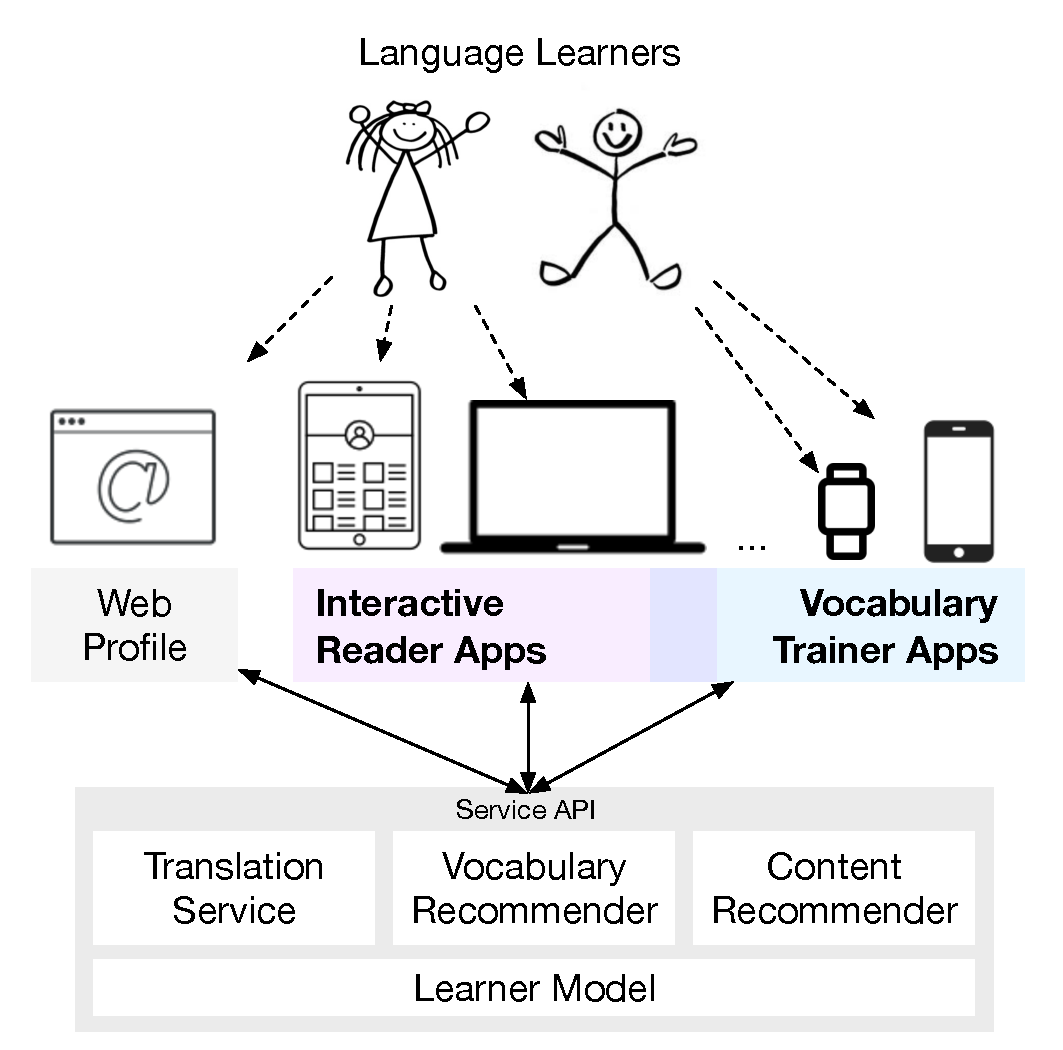
\includegraphics[width=0.7\columnwidth]{figures/zeeguu-architecture.pdf}
  \caption{The architecture of the envisioned software ecosystem}~\label{fig:architecture}
\end{figure}

\subsection{Learner Model}

The basic idea, sketched in Figure \ref{fig:architecture}, is that at the core of the ecosystem a ``learner model'' tracks the evolving knowledge of the learner. Based on this it can make recommendations to the individual applications. The individual applications, in turn, report back to the learner model events from which the learner progress can be infered. 


\subsection{Translator Service}

The core API of the ecosystem provides translations. It is critical that the translation service is used by all the applications in the ecosystem since this allows the server to track the words and the context in which they are being looked up. This information is then used for estimating learner knowledge and for generating personalized recommendations. 

The Translation Service is an API implemented using Python. Instead of implementing our own contextual translation engine, we decided to rely on existing industrial grade translation APIs. To avoid depending on a single service and to also increase the likelihood that at least one of the alternative translations is the correct one, the translation service dispatches in parallel requests to at least three third party translation APIs: Google Translate, Microsoft Translate, and Glosbe. \cite{Jager17-mux} The first two provide contextual translations and multi-word translations, while the third is a simple dictionary. 

The dependency of the translation service on multiple third party APIs allows for a higher reliability and a chance to guarantee a low response time: when a service is down or too slow to respond, the results from it are ignored. We detail elsewhere the strategies we use to keep response times low\cite{Jager17-mux}.

% by interacting with a core API that provides the basic contextual translations, user knowledge estimation, and recommendations for words to be studied and texts to be read \cite{Lungu16}. 

\subsection{Study Recommender}

There are two types of recommendations that an intelligent language textbook should make: 
\begin{itemize}
	\item Interesting and accessible texts to read. The texts should be both interesting and of an appropriate difficulty level to maintain the motivation. The current implementation of the text recommender allows the reader to select given online sources (e.g. news, blogs) which are interesting for them. The difficulty estimation of everytext is done by taking into account the frequency in the target language of all the words in the text. 
	\item Optimally-timed words to practice. To schedule the words to practice the system uses an adaptive, response-time-based scheduling algorithm [was developed] to increase the efficiency of perceptual learning by Mettler et al. \cite{Mettler14-ARTS}. After evaluating several alternative scheduling strategies we settled on the Mettler one since it has been proven to have gains with both familiar, seen items as well as with new, unseen instances and the benefits of adaptive scheduling were present at an immediate test as well as at a delay \cite{Mettler14-ARTS}.
\end{itemize}

% The scheduling algorithm is based on 


\subsection{A Web-Based Reader and Trainer Platform}



The system that we present in this paper as a {\em personalized language textbook} is composed of instantiations of the components. We present them in turn in this section, focusing the discussion on three key activities that a user of such an interactive textbook is interested in: 

\begin{enumerate}
	\item finding texts to read
	\item reading the found texts
	\item practicing vocabulary in context
\end{enumerate}

 % interacts with: the reader and the trainer applications. 
\begin{added}
	
	The system presented is implemented as a responsive web application, and thus can be used from a variety of devices. We also have implemented a trainer for smartwatch devices. However, in the experiments reported in this paper, it was used from Windows, Android, and iOS devices. 

\end{added}




%!TEX root=paper.tex

% \newpage
% \subsection{Web Article Reader}


    % A basic text reader should allow the learners to find interesting texts (e.g. news, blogs) and should provide a facile interaction for reading and translating unknown words. 
  
% The Web Article Reader allows the learners to subscribe to various sources of articles (e.g. news, blogs) and provides a facile interaction for reading and translating unknown words. 
% It consists of several components:

\subsection{Finding Personally Interesting and Accessible Texts}
% personally relevant vs. interesting... relevant can mean both interesting and not too difficult. 
% \ml{make sure that we use source consistently in the text; not feed for example.}
% From the user's point of view, the Reader is organized around {\em sources\xspace} of articles. The system categorizes sources by their language. 
The current system allows the learners to subscribe to various online sources (i.e. news, blogs) and then monitors those sources for new texts. Figure \ref{fig:system_subscriptions} presents the source subscription dialog listing multiple text sources for French.
% multiple sources for every language are pre-loaded in the system and if a reader wants to add a new source they have to send an email to the maintainers of the system. 



    \begin{figure}[h!]
    \centering
      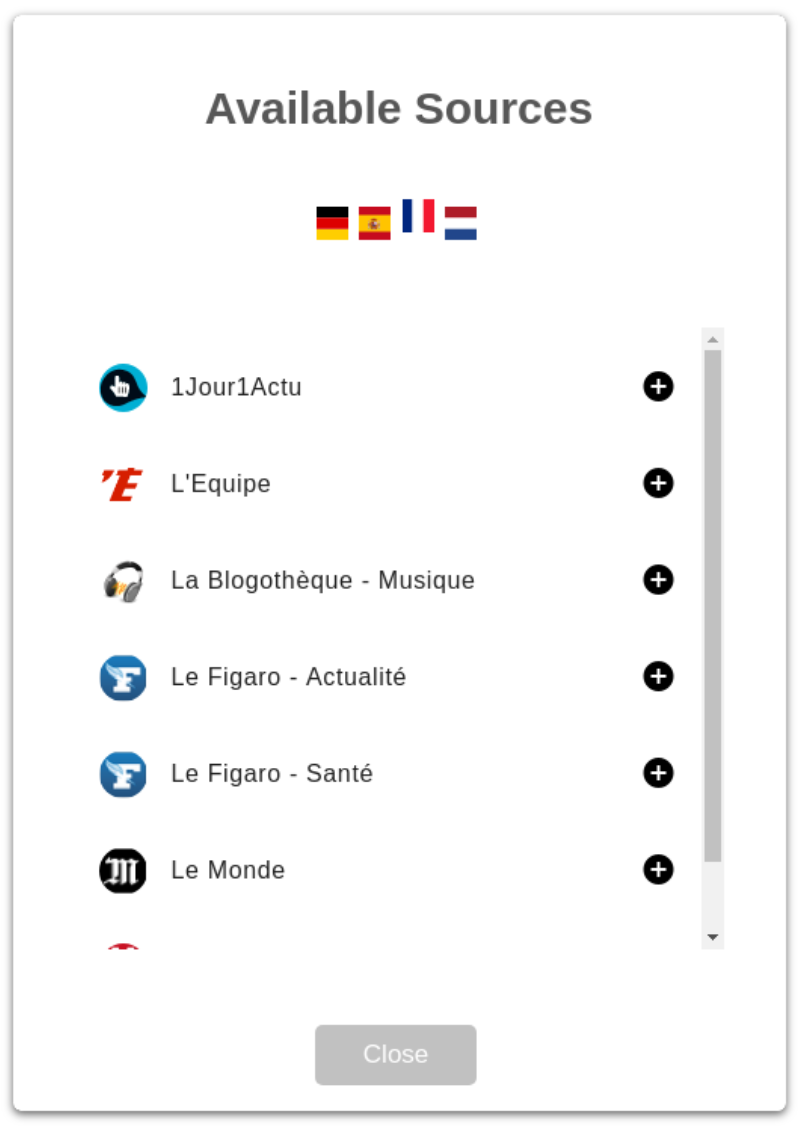
\includegraphics[width=0.3\columnwidth]{figures/available_sources}
      \caption{Different users subscribe to different sources}~\label{fig:system_subscriptions}
    \end{figure}

% A multi-lingual learner can subscribe to multiple sources in different languages. 
% \begin{added}

  Once a reader is subscribed to a source, that source is constantly monitored for new articles, which are recommended to the learner in an article browser like the one in Figure \ref{fig:article_listing}. The browser displays for each article an icon representing its source, a title, a summary, and an estimated difficulty level.
  To visualize the reading difficulty of an article, there are three levels of information displayed: 1) a flag representing the language of the article since a learner could be actually registered to feeds in multiple languages; 2) a color coded difficulty from green to yellow to red, to  allow the user to rapidly judge difficulty on an intuitive level; 3) a numerical difficulty score  to allow a more quantitative judgment of the estimated difficulty.
    
% \end{added}

    \begin{figure}[h!]
    \centering
      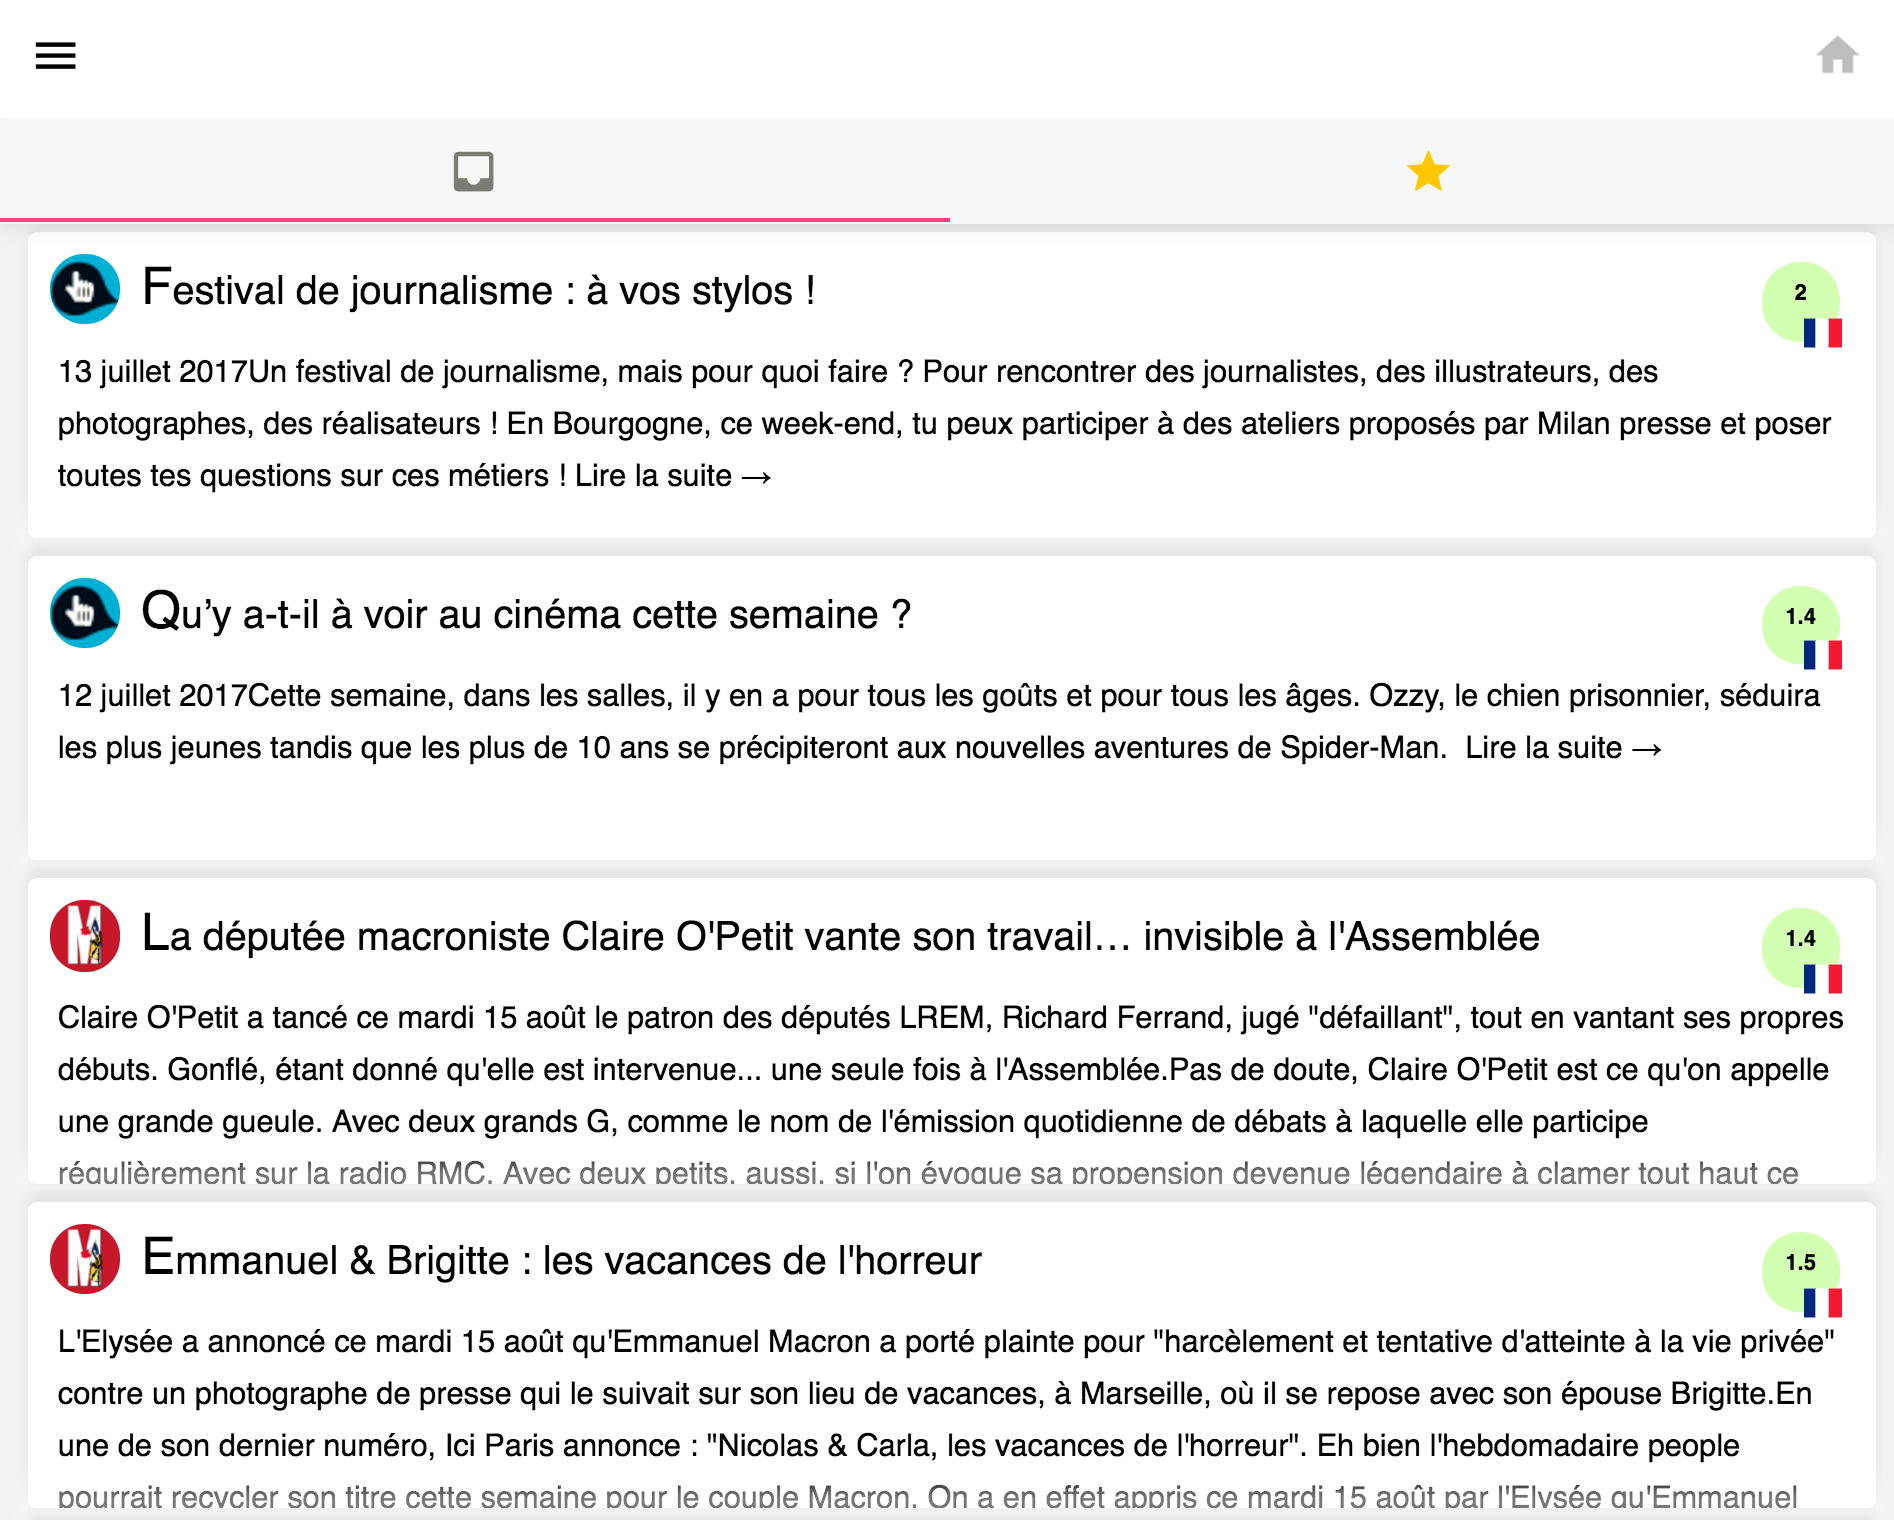
\includegraphics[width=0.75\columnwidth]{figures/article_listing}
      \caption{Article listing presents estimated difficulty levels }~
      \label{fig:article_listing}
    \end{figure}



Difficulty estimation takes into account the frequency of the vocabulary items in the text. The system filters out articles that are too difficult given that it was deployed with non-advanced learners.\footnote{This is one of the limitations of the system that we discuss later.}

\subsection{Interacting With Unknown Words While Reading}
% Reading Texts to Understand

To make reading as facile as possible, the reader is optimized for the most frequent action that a reader is likely to want to perform: translating a word. Thus, when a user clicks on a word, a translation is inserted right after the word, as Figure \ref{fig:translated_word} illustrates: 

\begin{figure}[h!]
\centering
  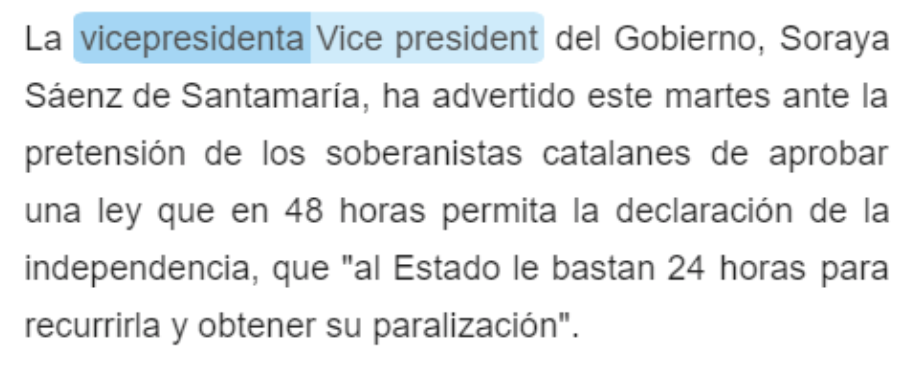
\includegraphics[width=0.7\columnwidth]{figures/translated_word}
  \caption{A translated word is inserted after the tapped word.}~\label{fig:translated_word}
\end{figure}

Two other alternatives that we explored and eventually dropped (for each had disadvantages) were: 

\begin{enumerate}

  \item Temporarily showing a popup of the translation and then hiding it again. This had a disadvantage for difficult sentences, where multiple words must be translated. The reader can forget translated words by the time they arrive at the end of an article, requiring them to re-translate.
  \item Using the native selection mechanism to select text as opposed to click / touch. 
  % We experimented with allowing the learner to select a word in the same way this is normally done on the corresponding platform. 
  This had the disadvantage that native selection is not designed as a priority action and thus is slow to respond (e.g. on Android a user must hold their fingertip down for almost a second before the contextual menu is displayed). 
\end{enumerate}


\subsubsection{Translating Multi-Word Expressions}

The user can chain a few consecutive words into a single translation by simply tapping adjacent words which are then automatically merged in a translation bubble (Figure \ref{fig:translation_extension}). This is useful for collocations and in cases where by expanding the translated set of words the precision of the translation increases. 

    \begin{figure}[h!]
    \centering
      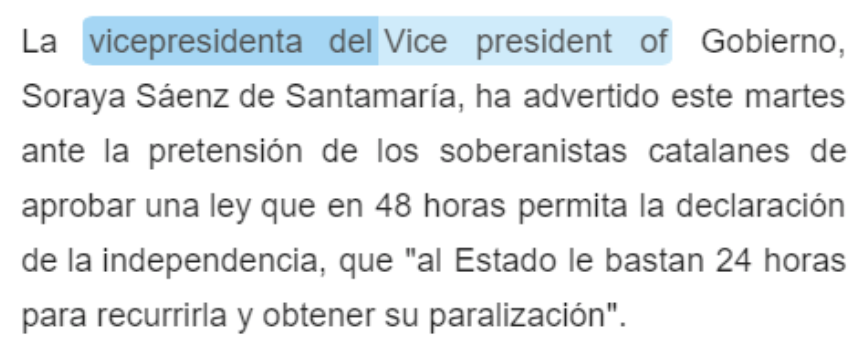
\includegraphics[width=0.7\columnwidth]{figures/translated_words1}
      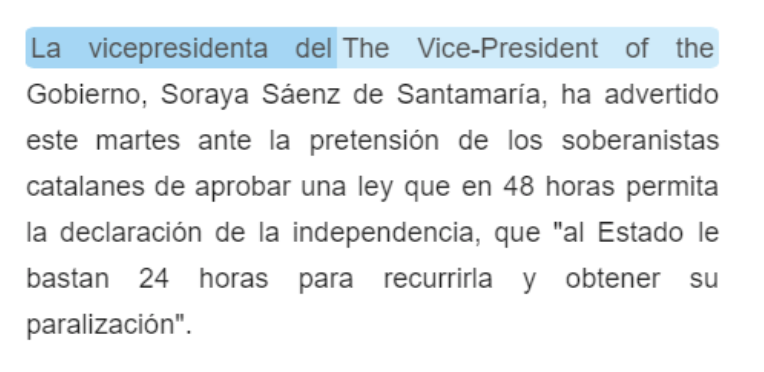
\includegraphics[width=0.7\columnwidth]{figures/translated_words2}
      \caption{When adjacent words are tapped the translation bubble is extended accordingly}~\label{fig:translation_extension}
    \end{figure}

This minimalistic interaction model serves a double purpose - it enables and eases the translation of several chained words but it discourages users from translating entire sentences or phrases. This is in line with the recommendations of the literature (e.g. Renandya argues that extensive reading should discourage intensive use of translations\cite{renadya07-power}) but also because it reduces the amount of characters which are being translated by the learner (and thus the costs of the system, since some of the translation services have a per-character fee). 

One of the limitations of this interaction is that it is not clear (at least at the moment) how to expand it for the situations in which expressions are present that are composed of words which are not adjacent (e.g. particle verbs in German).


\subsubsection{Compensating for the Limits of Machine Translation}
Due to the limitations of machine translation multiple translations might be possible in a given context. In such a case the system will insert the most likely alternative as described earlier right after the selected text, but it will allow the reader to discover alternatives. With a click on the translation, a drop-down menu appears in which alternatives are presented. Figure \ref{fig:registrations} shows that besides the predefined alternatives the learner can provide their own translation via an input box (the third line, ``took place'' is typed in by the learner in the figure). 


\begin{figure}[h!]
\centering
  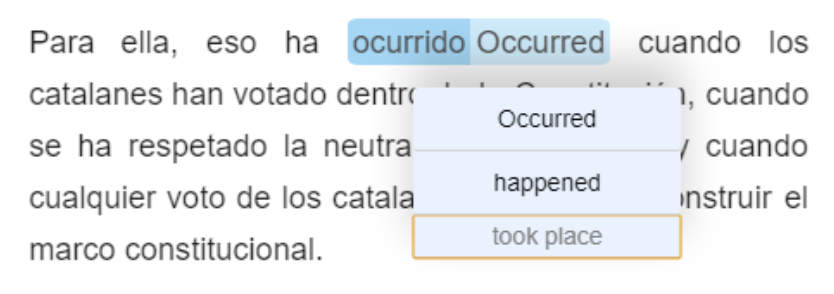
\includegraphics[width=0.7\columnwidth]{figures/translation_alter_menu}
  \caption{A translated word is inserted after the tapped word.}~\label{fig:registrations}
\end{figure}

\subsubsection{Discovering the Pronounciation of a Word}

The process we followed while developing the reader was an iterative process, with short release cycles (one or two weeks), and frequent testing with members of the research team, and the occasional external user. 

One of the features that we added following a suggestion of an early beta-tester -- a teacher of Dutch as a foreign -- was the pronounciation of a translated word. After exploring several trade-offs between flexibility, ease of use, and a clean user interface, we settled on triggering the pronounciation of a word (or group of words) with a tap. 

% The pronounciation is generated by using the HTML5 Speech API which is supported by most modern browsers both on the mobile and on the desktop. 

% \ml{could ask the users if they are happy with it.}
% Although no user has yet complained about it, this means that a user can not pronounce a word without it being translated first. It might also be that for some languages this is more important than for others, and we just did not have users learning those languages (e.g. Danish is notoriously hard to pronounce). In the future we plan to expand the interaction modes to allow pronounciation to exist seperately from translation.
%!TEX root=paper.tex

\newpage
\subsection{Web Vocabulary Trainer}

Given the list of words that a user does not know since they were looked  up in the past we can generate exercises for they user.

Figure \ref{exercise_translate} shows such a generated exercise which asks the reader to translate a given word in the context in which it was encountered in a past reading. The main interactive elements (IEs) that are specific to this exercise are an input box that allows the user to enter a solution (IE5); a button for checking the correctness of the input answer (IE2); a hint button which presents the correct answer (IE1). Two types of control that span exercise types are: a word pronunciation option (IE3) and a feedback option (IE4) which allows the user to provide feebdack about the exercise.

\begin{figure}[h!]
\centering
  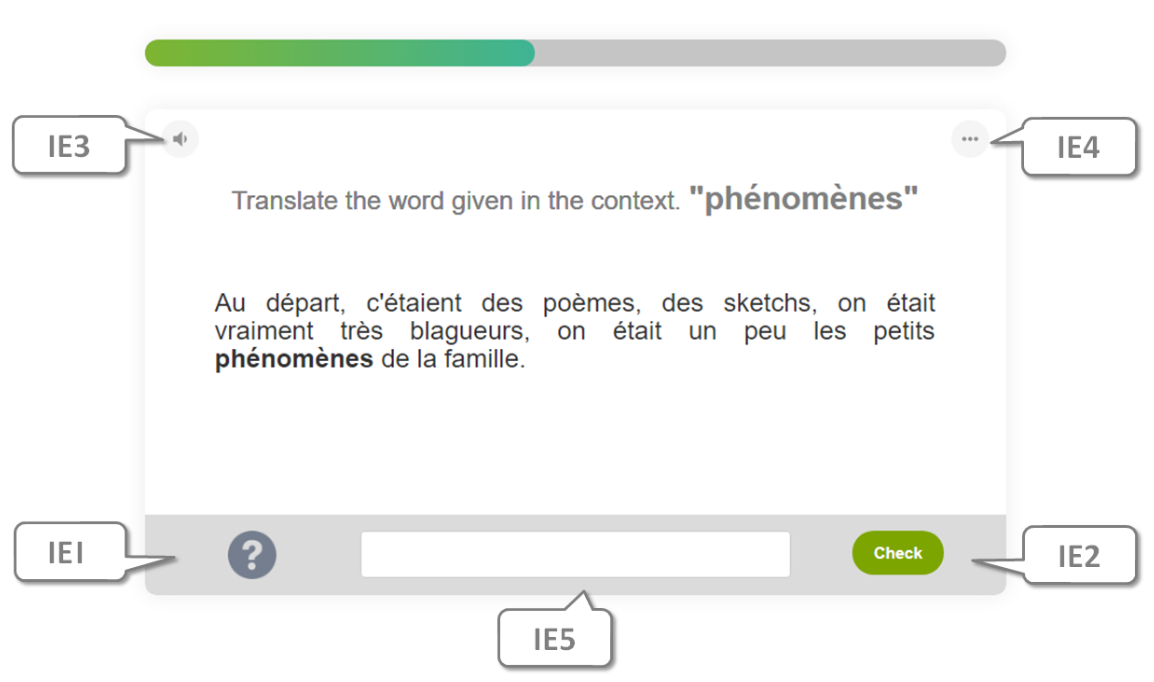
\includegraphics[width=0.9\columnwidth]{figures/exercise_translate}
  \caption{One of the exercise types with which the user is presented asks the user to translate a word in a context that is retrieved from the user's past readings}{
  \label{exercise_translate}
  }
\end{figure}

\ml{The system currently implements three other types of vocabulary practice exercises: one similar to the one in figure, but where the user has to select one of three possible translations, one where the user has to translate to the learned language, not to his known language. A third type of exericse asks the learner to match translations to originals}.

\subsubsection{Selecting Words to Study}

Since a learner might encounter many words that are not understood, we need to prioritize those that are to be studied in exercises. We use three aspects to prioritize words: 

% The words good for study are the ones that are either starred by the user, or are important and of quality based on a set of heuristics. 

\begin{description}

  \item [Important Words] are the ones which appear frequently in the language. For word frequencies we use frequencies computed based on movie subtitles which have been shown to be highly representative to frequencies in human interacitons \cite{New07-subtitles}. 
  
  \item [Quality Context] we favor words that come with a context which is not too short but not too long. 

\end{description}

\subsection{Study Recommender}

The scheduling algorithm is based on an adaptive, response-time-based scheduling algorithm [was developed] to increase the efficiency of perceptual learning by Mettler et al. \cite{Mettler14-ARTS}. After evaluating several alternative scheduling strategies we settled on the Mettler one since it has been proven to have gains with both familiar, seen items as well as with new, unseen instances and the benefits of adaptive scheduling were present at an immediate test as well as at a delay \cite{Mettler14-ARTS}.



% \subsection{Translator Service}

% The core API of the ecosystem provides translations. The main advantage of this indirection is that this allows the server to track the words that are looked up and the context (sentence) in which they are being looked up. This information is then used for estimating learner knowledge and for generating personalized exercises. 

% The Translation Service is an API implemented using Python. Instead of implementing our own contextual translation engine, we decided to rely on existing industrial grade translation APIs. To avoid depending on a single service and to also increase the likelihood that at least one of the alternative translations is the correct one, the translation service dispatches in parallel requests to at least three third party translation APIs: Google Translate, Microsoft Translate, and Glosbe. \cite{Jager17-mux} The first two provide contextual translations and multi-word translations, while the third is a simple dictionary. 

% The dependency of the translation service on multiple third party APIs allows for a higher reliability and a chance to guarantee a low response time: when a service is down or too slow to respond, the results from it are ignored. We detail elsewhere the strategies we use to keep response times low\cite{Jager17-mux}.


% \begin{figure}[h!]
% \centering
%   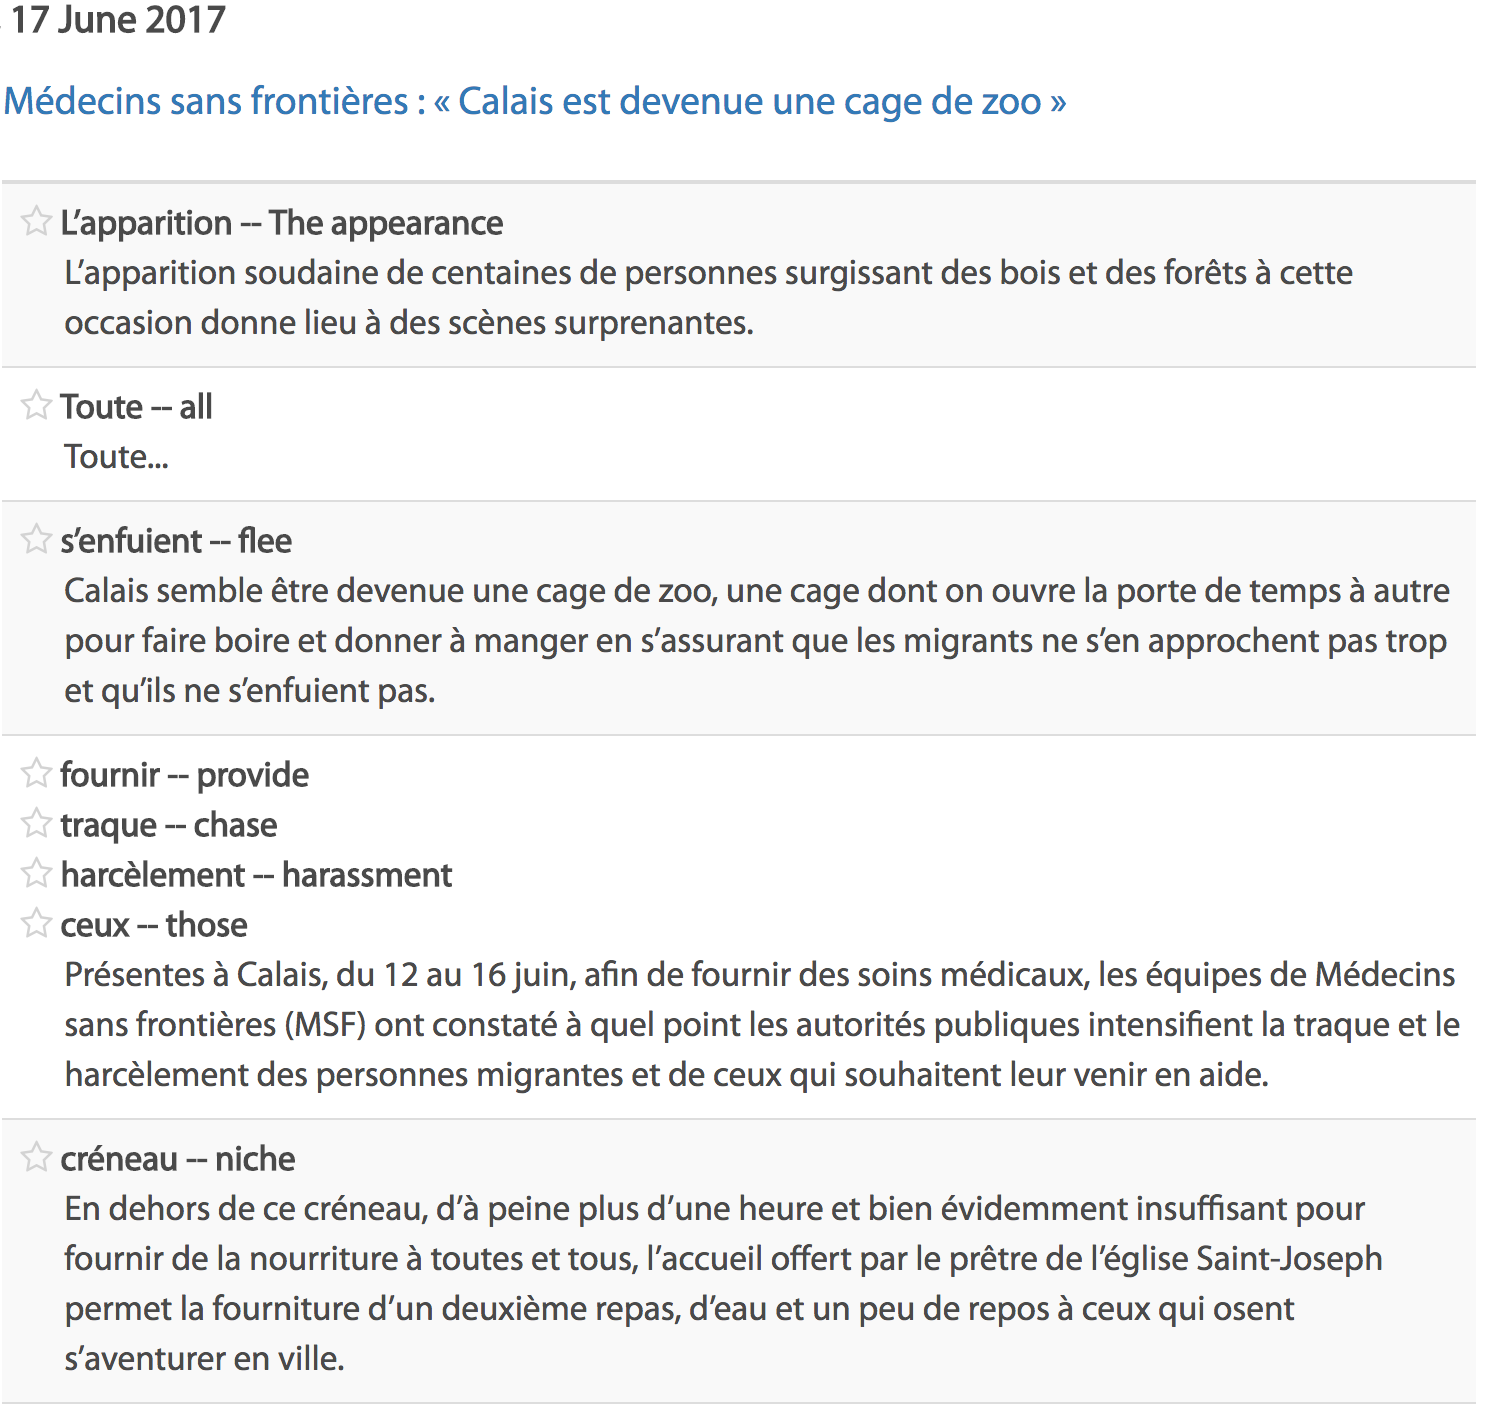
\includegraphics[width=\columnwidth]{figures/teacher_dashboard.png}
%   \caption{A teacher can see the log of the words that a student looked up, their chosen translations, and the corresponding contexts}{
%   \label{fig:teacher}
%   }
% \end{figure}





%!TEX root=paper.tex

\newpage
\section{Testing With High School Students}
\label{sec:demographics}

We tested our system with \stcnt students from a public highschool in Groningen, The Netherlands. They represent three classes that have the same French teacher and are bilingual in Dutch and English. At the beginning of June 2017, we visited the school, and during one hour in each of the three classes we introduced the tools and their usage.

The system was used officially in class from the second week of June until the end of the month (coinciding with the end of the semester). With few exceptions the students created an account and started using the system the latest on June 9th. 

The teacher asked the students to use the infrastructure as much as they liked and to write reports on their activity. For every half an hour of usage, the students had to write a brief report on how they spent their time and submit it to the teacher. The teacher could then decide to selectively test them on the basis of their reports.

We deployed the system with the translations from French to English instead of Dutch since, based on our experience translation APIs are of higher quality when one of the languages is English and because the students and their teacher were comfortable with the idea.\footnote{We made it clear to the students that they can ask us, and we will modify their personal account in such a way as to receive translations in Dutch. None of the students requested this.}

We also invited the students to send us feedback at any time if they encounter problems or if they have ideas for improvement. Several of them did email. Towards the end of the month, we also deployed several in-app focused pop-up questions using a customer opinion elicitation service called HotJar. After the month was over we sent out a follow-up questionnaire.

\subsection{Demographics}

Before creating accounts on our platform, the participants were directed to a survey form which asked them to provide personal information about their current level of knowledge, learning strategies, and interests. A handful of the participants did not fill the survey before using the system.

The participants that filled our survey were 54 female and 15 male with ages below 18 representing three different classes. Based on their own self characterization, 53 students are level B1 (i.e. can understand the main points of clear standard speech, can narrate an event, an experience or a dream) and 16 are level A2 (i.e. using simple words, can describe their surroundings and communicate immediate needs). 


When asked whether they have favorite topics they would like to read about, half of the students mentioned various topics while the other half did not answer the question. From the topics that they mentioned as possible interests some of the more popular were: sports, music, travel, lifestyle, fashion, movies, and somebody mentioned as interest {\em ``no politics''}.

We seeded the system with a variety of French news and blogs that cover these aspects: 1Jour1Actu, L'Equipe, La Blogoteque, Le Figaro, Le Monde. 











% To talk to Nienke about the other types of analysis we can do on this data
%!TEX root=paper.tex

\newpage
\section{How Do Students Use the Possibility of Reading Personally Interesting Articles?}
\label{sec:results}

% \subsection {Feed Subscriptions}
Figure \ref{fig:registrations} represents an incidence matrix collected at the end of the study interval: the columns represent students, and the rows represent news feeds; if a student is registered to a given feed, at the intersection of the corresponding row and column we place $\Diamond$. 

We would expect to see fully continuous horizontal rows of data-points if every user subscribed to the same feed, and fully continuous vertical rows if every user subscribed to all of the feeds available. The notion that these patterns are largely absent in Figure 4 supports our assumption that different individuals prefer to subscribe to different reading sources.

The figure illustrates that giving the students the freedom to choose the sources they wanted, allowed each one of them to express their interest. 

\begin{figure}[h!]
\centering
  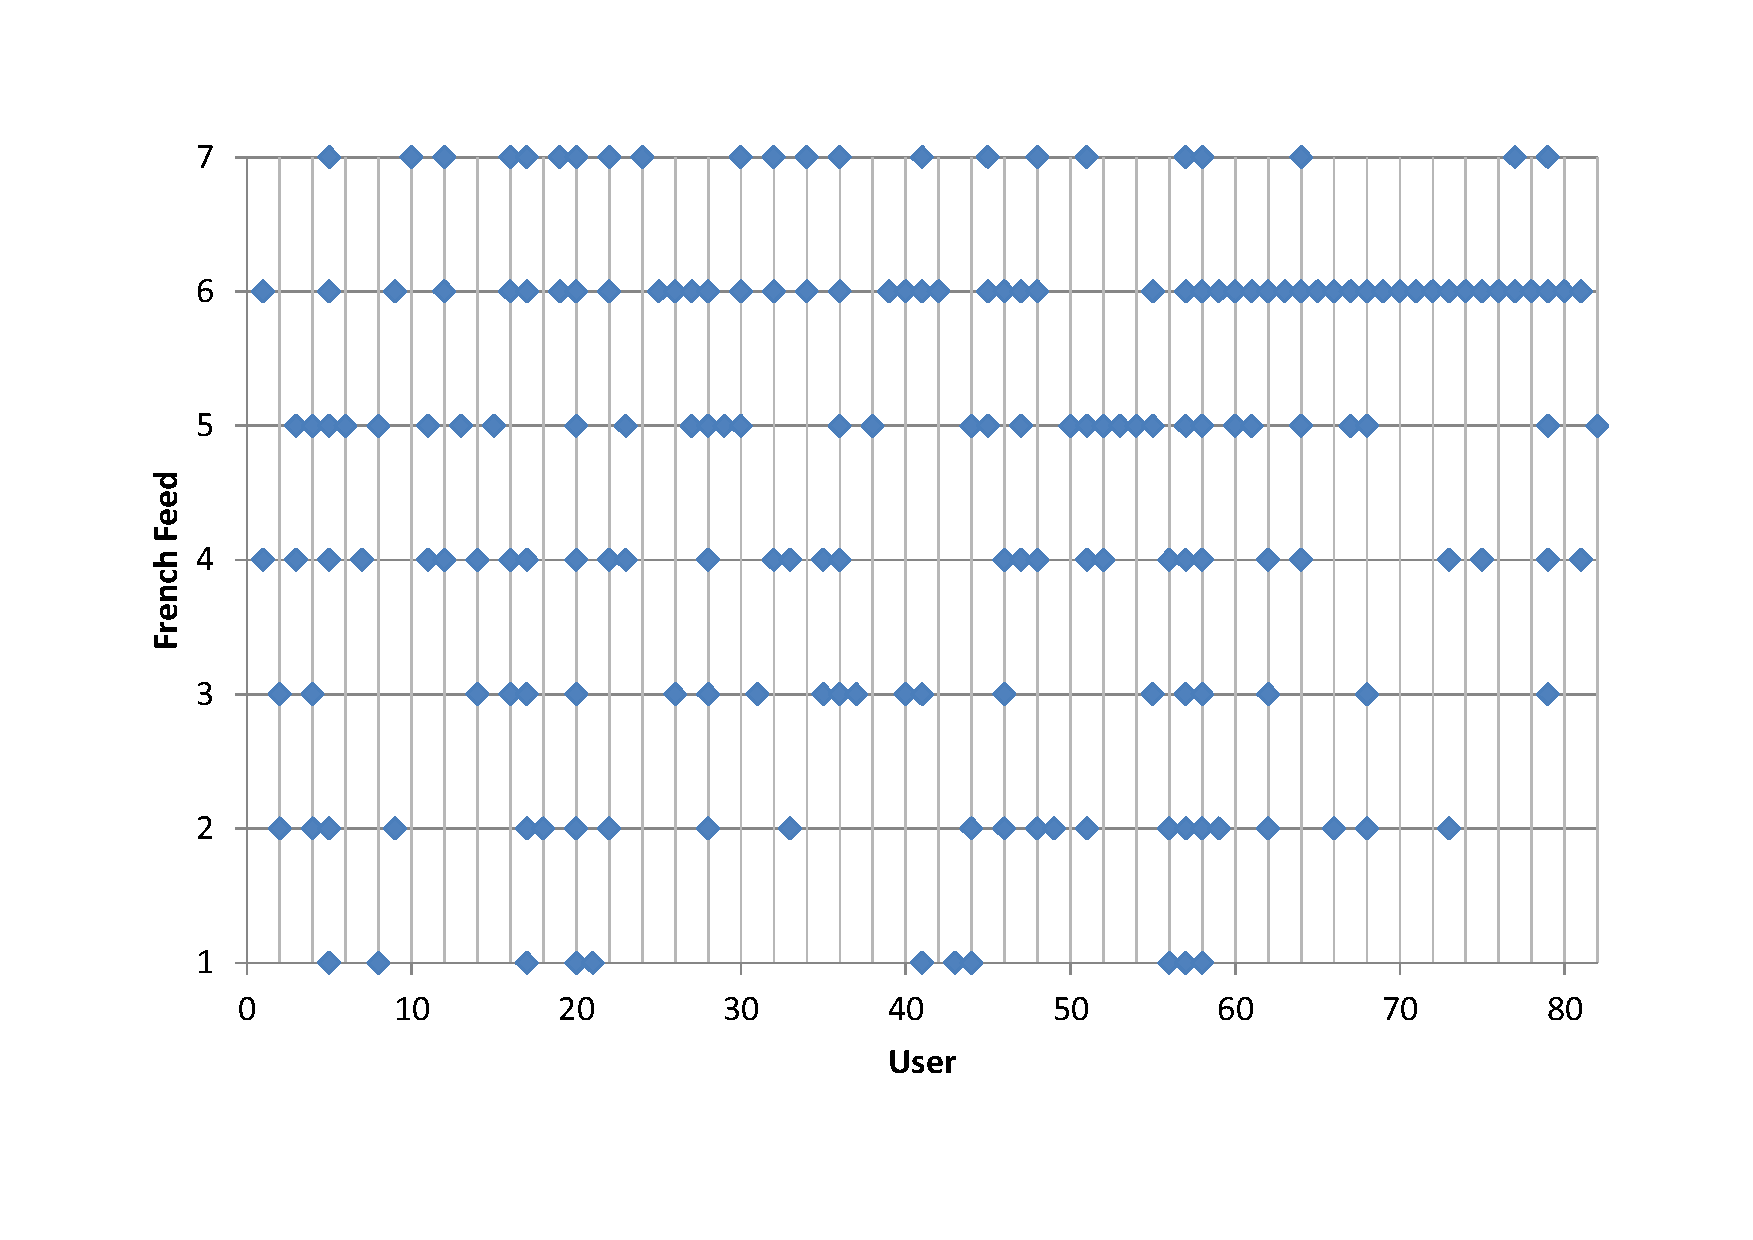
\includegraphics[width=\columnwidth]{figures/users_feeds}
  \caption{Different users subscribe to different sources}~\label{fig:registrations}
\end{figure}

Of course some feeds are more popular than others. Projecting the data- points into the vertical axis and sorting the results leaves us with a histogram as can be seen in Figure 5.

\begin{figure}[h!]
\centering
  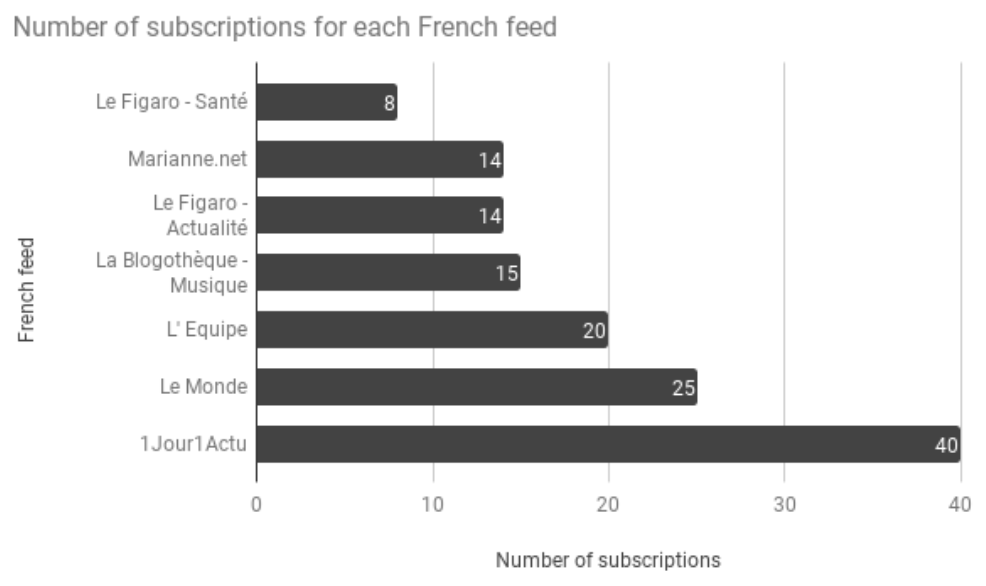
\includegraphics[width=\columnwidth]{figures/feed_popularity}
  \caption{Some feeds are more popular than others}~\label{fig:registrations}
\end{figure}


Feed {\em 1Jour1Actu} is the most popular French feed, and feed Le Figaro - Sant\'e is the least popular French feed. In order to see whether or not this might be related to how they are presented in the dialog window of our system (see Figure \ref{fig:system_subscriptions}), we can compare the order of popularity with the order in which they are displayed.

\begin{figure}[h!]
\centering
  \newcommand{\picscale}{0.5}
\begin{tikzpicture}[scale=\picscale, every node/.style={scale=\picscale}]
    % Columns.
    \node at (0  , 0) {\bf Presented};
    \node at (2.5, 0) {\bf VS};
    \node at (5  , 0) {\bf Popularity};
    
    % As presented.
    \node at (0,-1) {1Jour1Actu};
    \node at (0,-2) {L'Equipe};
    \node at (0,-3) {La Blogoth\`{e}que};
    \node at (0,-4) {Le Figaro - Actualit\'{e}};
    \node at (0,-5) {Le Figaro - Sant\'{e}};
    \node at (0,-6) {Le Monde};
    \node at (0,-7) {Marianne.net};
    
    % As popular.
    \node at (5,-1) {1Jour1Actu};
    \node at (5,-2) {Le Monde};
    \node at (5,-3) {L'Equipe};
    \node at (5,-4) {La Blogoth\`{e}que};
    \node at (5,-5) {Le Figaro - Actualit\'{e}};
    \node at (5,-6) {Marianne.net};
    \node at (5,-7) {Le Fiaro - Sant\'{e}};
    
    % Arrows between presented and popular.
    \draw [->] (1,-1)   --   (4,-1);
    \draw [->] (1,-2)   --   (4,-2.8);
    \draw [->] (1.2,-3) --   (3.7,-3.9);
    \draw [->] (1.6,-4) --   (3.4,-4.9);
    \draw [->] (1.4,-5) --   (3.7,-6.9);
    \draw [->] (1,-6)   --   (4,-2.1);
    \draw [->] (1.2,-7) --   (3.9,-6);
    
\end{tikzpicture} 
  \caption{The popularity of the feeds vs. their ranking in the UI}~\label{fig:registrations}
\end{figure}

One can see how the second-to-last presented feed, Le Monde, is the second most popular feed by measure of subscriptions. Conversely, the feed listed above Le Monde is actually the least subscribed-to feed in our listing.

\subsection{Article Interactions}
If we investigate the articles that the users interact with, we see the same pattern: each user explores their own interest, and there is no one article that is interesting for all of them. \ml{Can we provide a bit more information: which article is read by the most people, and how many people is that? Maybe we could sort this not by article ID, but reorder the article lines, in such a way that the most popular ones are at the bottom and the most unique ones at the top?}

\begin{figure}[h!]
\centering
  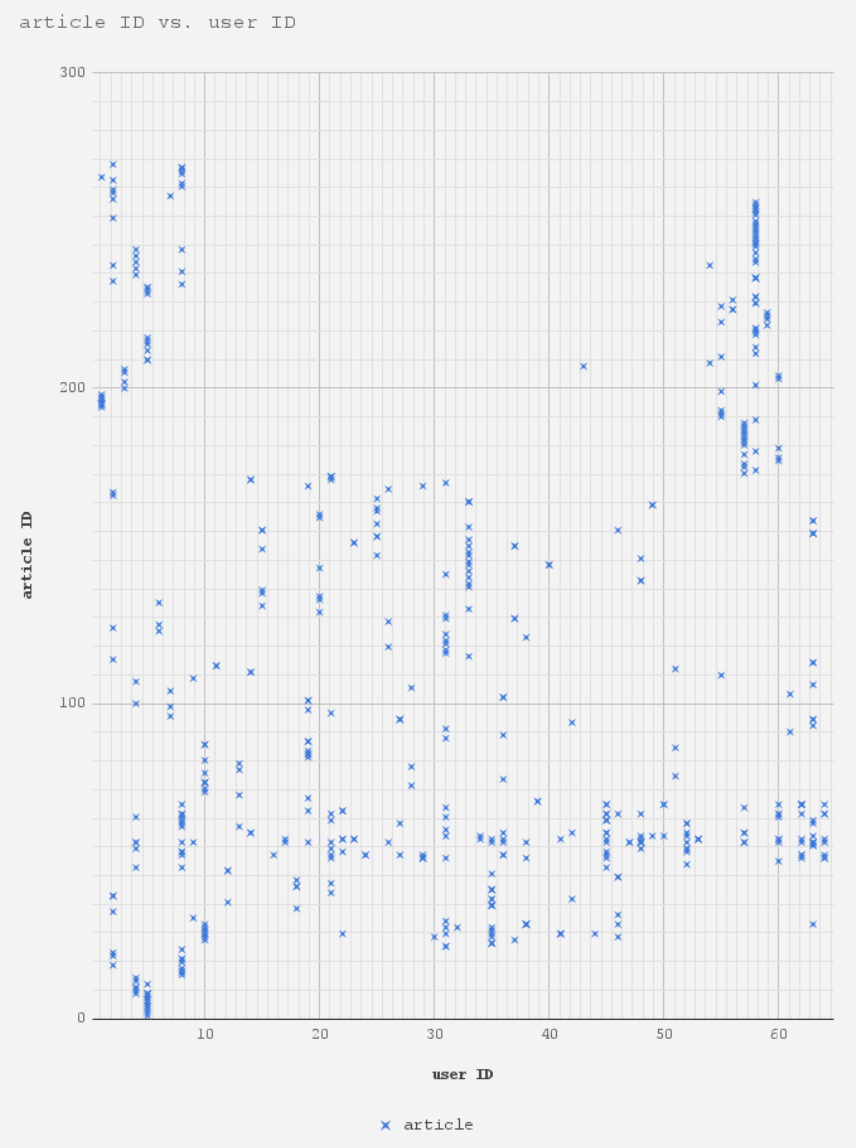
\includegraphics[width=0.8\columnwidth]{figures/users_articles}
  \caption{Every student has their own article reading preferences}~\label{fig:registrations}
\end{figure}

\subsection{Which Interactive Features Are Most Used?}
We tracked the usage of the various features in the interactive reader through a telemetry system that records all the interactions with a set of interactive elements of interest. Figure \ref{fig:feature_usage} shows the most used features of the system. With 6700 occurrences, requesting a translation for a word is the most used interactive feature of the system. The second most used feature is opening the ``translation alternatives'' menu. The ratio of translations to alternate translation requests is six to one. 

The third most used feature is the text to speech feature. On average, there are about 1.66 pronunciations for a given selection, suggesting that users are often asking for a second pronunciation after hearing it the first time. \ml{@dan, do you agree with this conclusion? it's opposite to your thesis, but I think it's correct}

Undo-ing a translation is used when the user wants to remove the translation that he just added to the text. This seems to be a very popular action too. 

A {\em like} button found at the bottom of an article  was clicked by the readers 174 times. Although currently this information is not used in a feture, it can be used to improve text recommendations and to add a social dimension to the system by providing information about how other people reacted to a given article.

\begin{figure}[h!]
\centering
  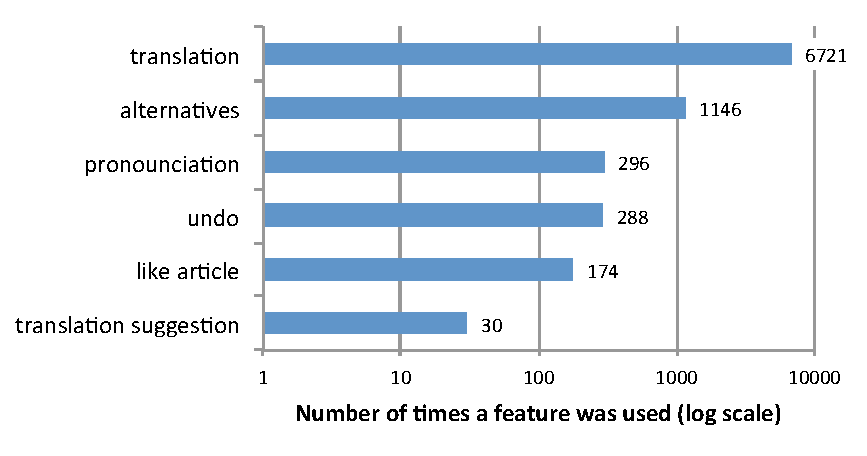
\includegraphics[width=0.9\columnwidth]{figures/reader_feature_usage}
  \caption{Popularity of features by their recorded usage-events}
  \label{fig:feature_usage}
\end{figure}

% \ml{like -- what does it mean for design? can we verify that they actually read those articles. how many did they read and didn't like?}

To see how widespread the various features are among our users, we also looked at the number of distinct users for each category of events. A larger number of distinct users indicates that the feauture is useful to the broadest number of students.

The least used feature presented in the Figure \ref{fig:feature_usage}, {\em translation suggestion}, allows users to contribute their own translations when they are not satisfied with the one automatically offered by the system. We see that the feature was used thirty times.  \ml{which brings me to: @Dan, what do you mean by alternatives here? :) Is it the number of times somebody selected an alternative, or the number of times they opened the menu. In any case, can we get the other number?}

\begin{figure}[h!]
\centering
  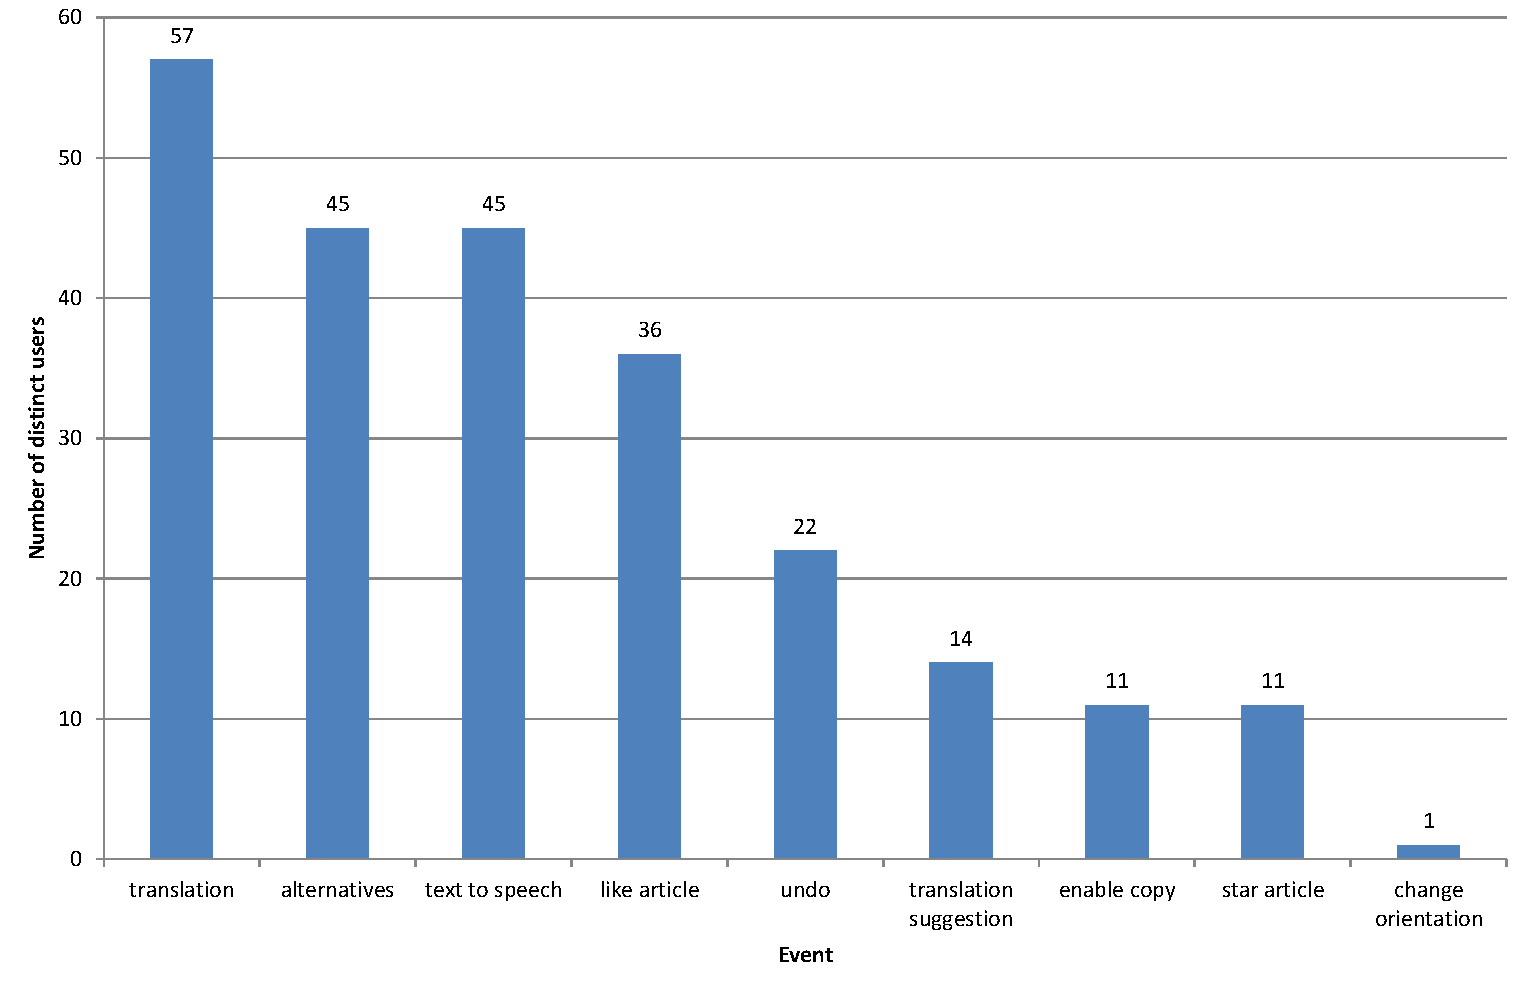
\includegraphics[width=0.9\columnwidth]{figures/reader_feature_usage_per_user}
  \caption{The usage of the various reader features by the various users }
  \label{fig:usage_per_user}
\end{figure}

In addition, we looked at the number of times the same word or phrase was pronounced by the same user. This data ranges from one single pronunciation to 14 pronunciations for the same word (phrase). The size of this interval is mostly due to the users' different proficiency in a certain language and the difficulty in pronunciation of the word (phrase) itself. Nevertheless, on average, the number approaches 1.66 pronunciation requests for the same
piece of text, suggesting that users are generally sufficiently content with a pronunciation after hearing it the first time.



\section{How Do Students Use the Personalized Vocabulary Exercises?}

The personalized exercises are a complement to the reading. 

The system presented four types of vocabulary practice exercises to the students. In total, during the entire duration of the study we observed 18.082 exercises being presented to the students, leading to an average of 300 exercises per student. Figure \ref{fig:ex_interactions} shows one outlier student who did 3.000 (!) exercises during one month, and about six over-eager students who did close to 700 exercises. 

The figure also highlights the difference between exercises which had a ``correct'' outcome vs. exercises which had a ``wrong'' outcome. 


  \begin{figure}[h!]
  \centering
    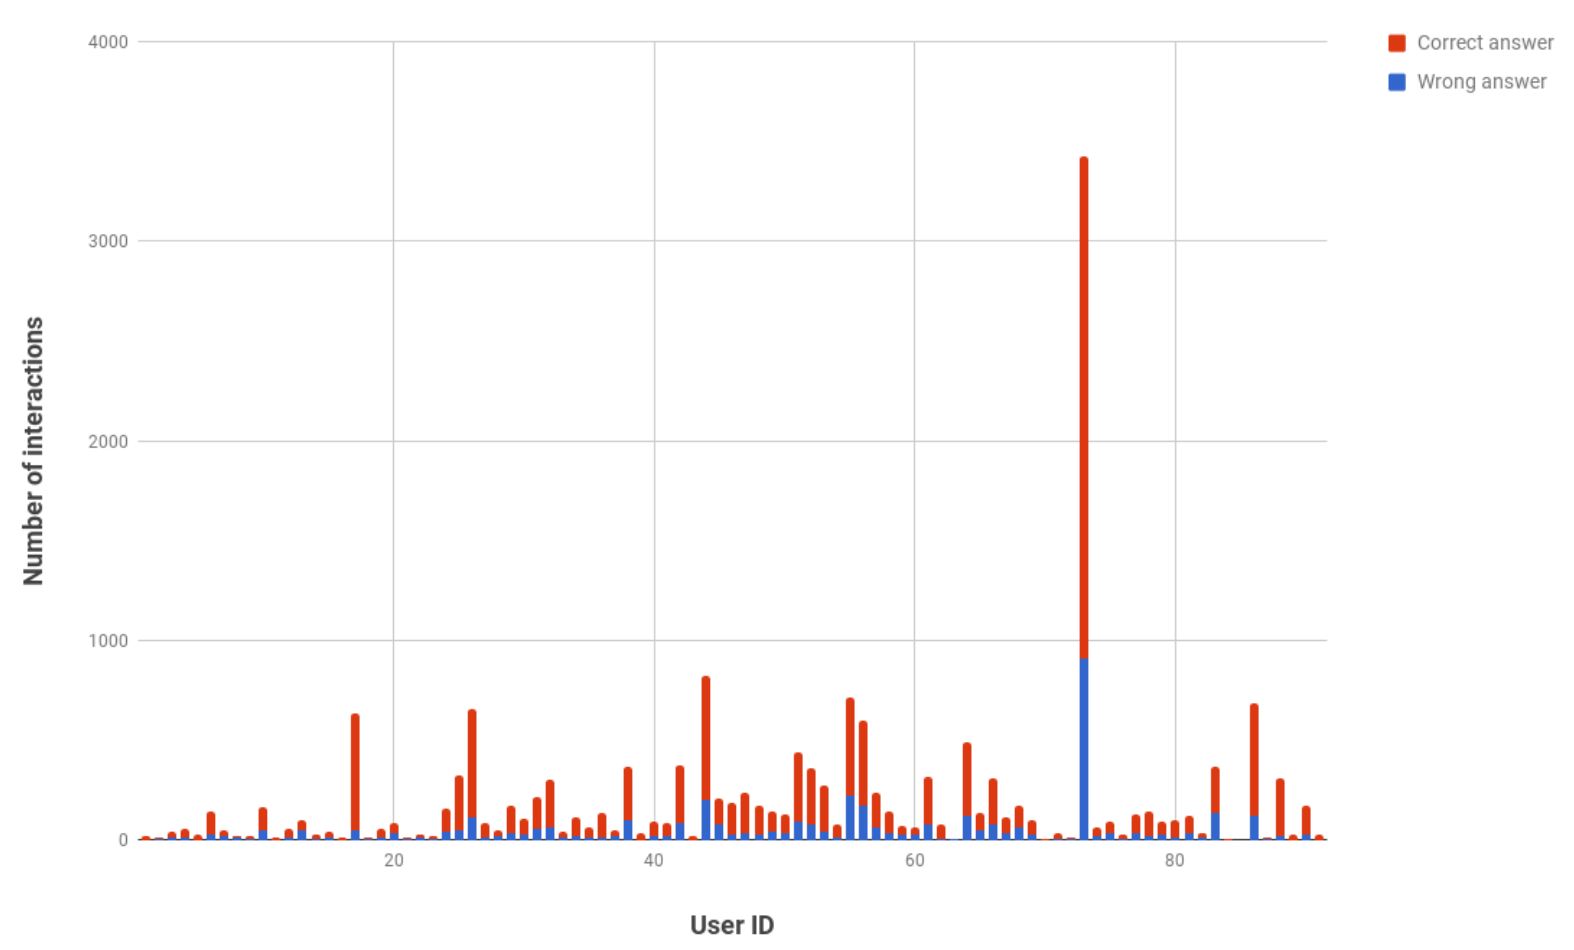
\includegraphics[width=\columnwidth]{figures/exercise_interactions_count.png}
    \caption{Some students are much more motivated than others in doing exercises }
    \label{fig:ex_interactions}
  \end{figure}


% \begin{tabular}{lrrrr}
%   % source id: 
%   % choose -- 5
%   % find -- 4
%   % translate -- 7
%   % match -- 6
%                       & Choose  & Find & Translate & Match \\ \hline
%   Total interactions  & 7180    & 6249 & 2643      & 2010\\
%   Hint requests       & 29      & 529  & 847       & 16 \\ \hline
% \end{tabular}

Figure \ref{fig:activity_per_day} shows in which days are the individual learners using the exercises. What we see is a distribution over the entire period of the study, with a slightly more intensive period towards the end of the period which might signify cramming before the end of the semester.

  \begin{figure}[h!]
  \centering
    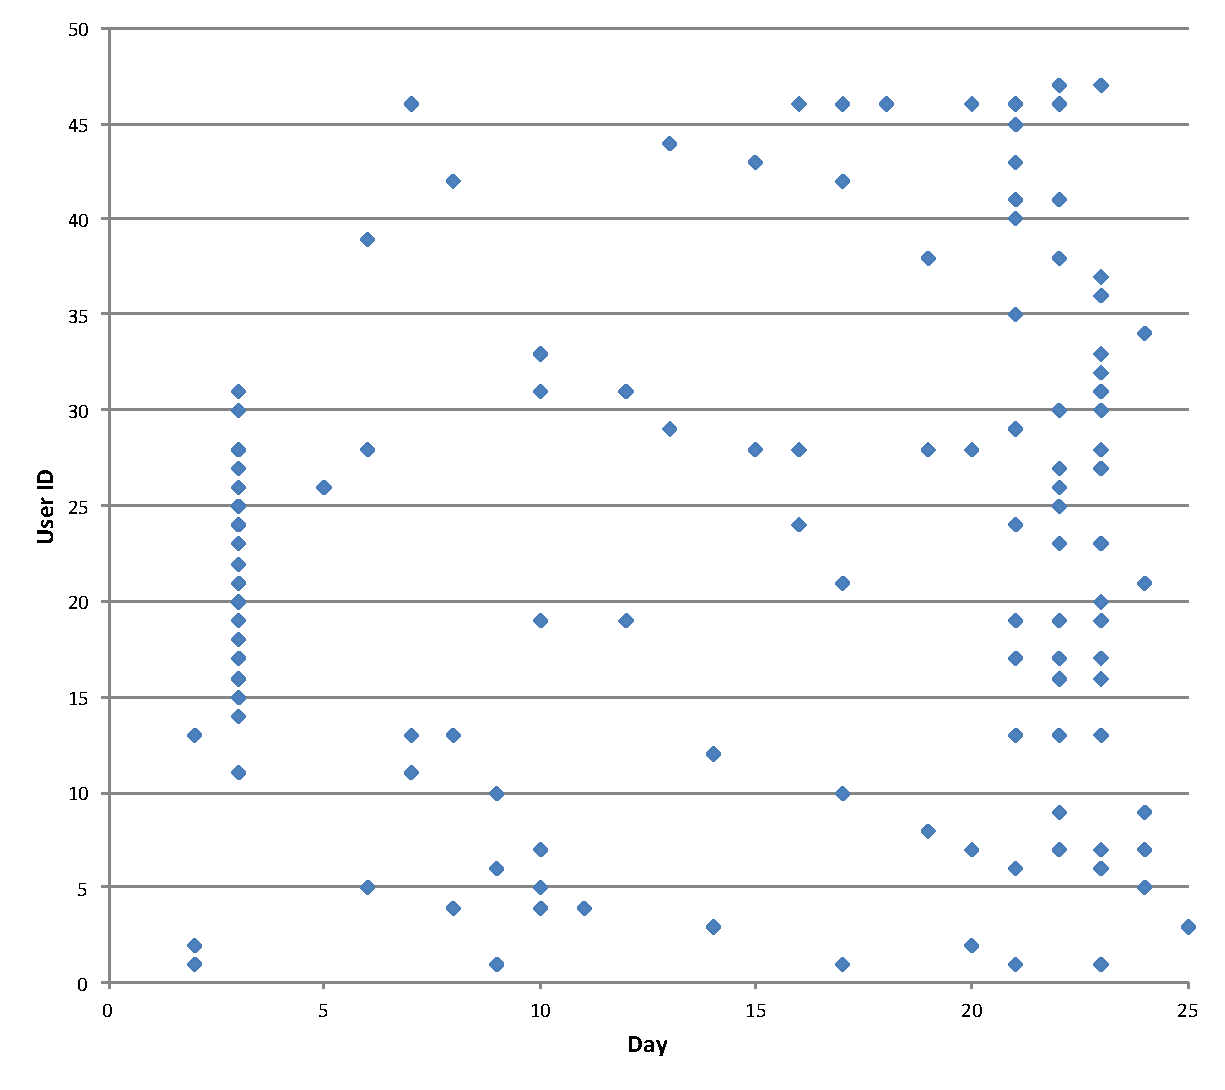
\includegraphics[width=\columnwidth]{figures/user_exercise_activity_vs_day.pdf}
    \caption{The students are doing exercises at their own pace throughout the one month interval }
    \label{fig:activity_per_day}
  \end{figure}

\newpage
\section{What is the Perception of the Learners?}

\subsection{In App Feedback Request}
Besides the analysis that we did based on the observed user data, we also asked the students a series of questions by popping up questions while they are using the sytem (by using an online tool called HotJar). Among the questions was whether they preferred the reading platform and why. Some of the qnswers can be seen in the screenshot below. It becomes clear that the students appreciate the possibility of reading what is interesting for them.

    \begin{figure}[h!]
    \centering
      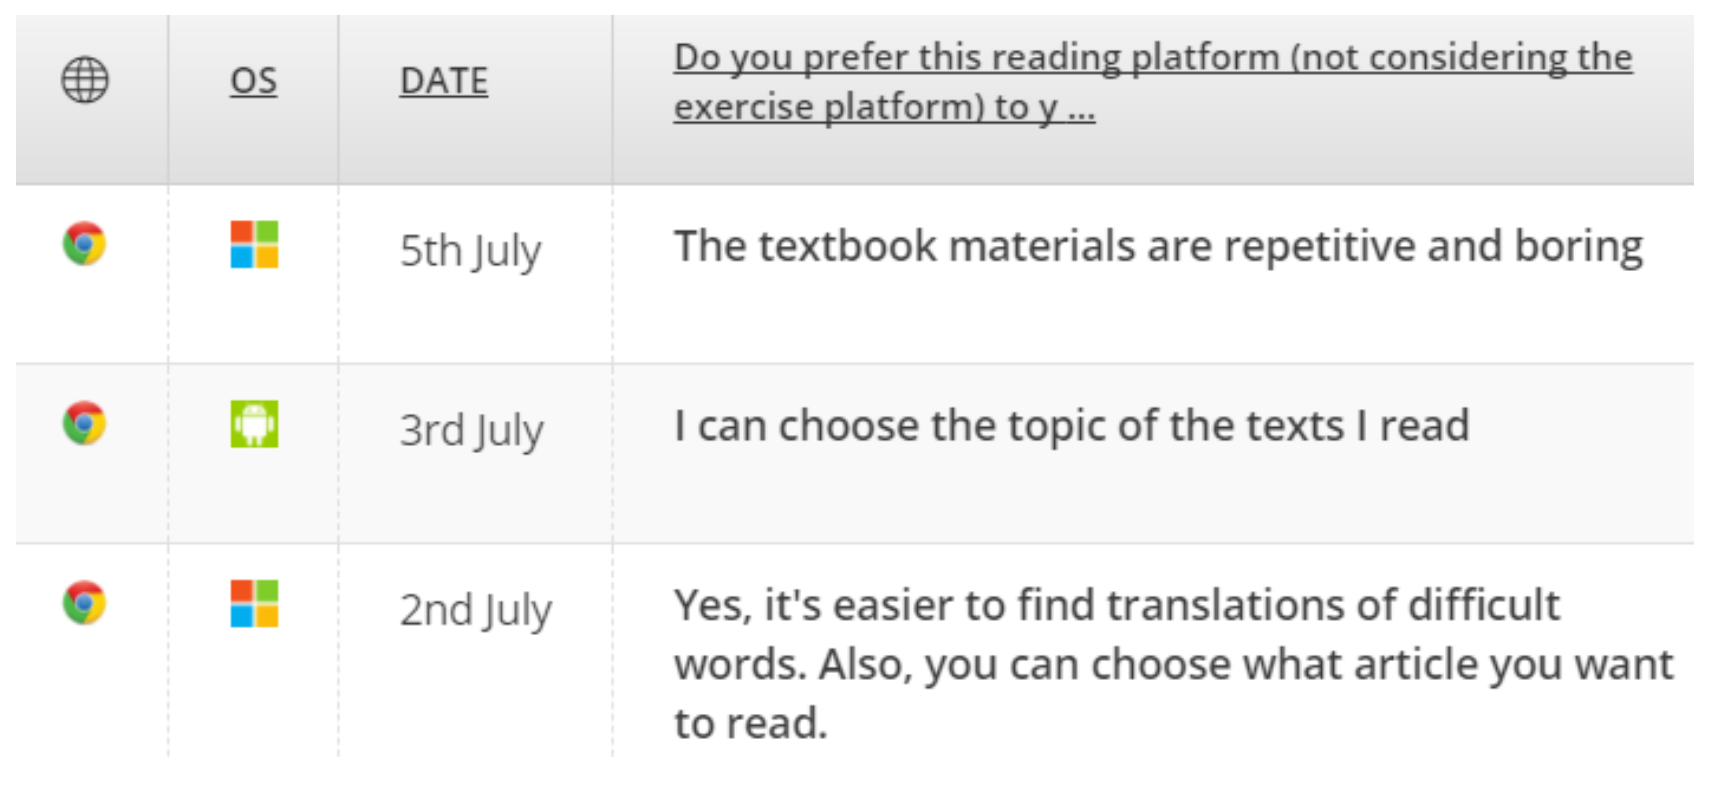
\includegraphics[width=0.9\columnwidth]{figures/opinion_on_reading_platform}
      \caption{The students appreciate the freedom of reading what is interesting to them }
    \end{figure}

\subsection{Post-Usage Survey}

The majority of the students who answered our post-usage survey said that  they prefer our system to a textbook. However, we still think this is not very conclusive since the number of students who answered our survey was quite limited: 12 of the 60 students represent about 20\% of the participants. 


\subsection{Reports to the Teacher}
However, since they might have been more sincere when reporting to their teacher than directly to us, we report here also what they wrote in a separate evaluation of the tools they use in the class, which the teacher runs always at the end of the school year. Several of the answers are: 

\begin{description}
  \item {\em ``It works well but it were better if the translation would have been in Dutch. It is good that you can choose yourself what to read.''}
  \item {\em ``Good for reading skills. It would have been best if it were in Dutch.''}
  \item {\em ``Your vocabulary is really moving forward, but then you have to do it more often than a few times. Overall a nice website, easy and fun subjects''}
\end{description}

There main message in the feedback is that learners appreciate the freedom of chosing materials to read that are personally interesting for them. The second, implied observation is that they appreciate the translations, but they would want to have them in their native language. 

% The way forward is then, by providing better recommendations if possible, and by providing translations in their native languages.

% In the future we plan to investigate whether the system works well enough with Dutch.

\newpage
\section{Limitations of this Study}
\label{sec:limitations}
% We presented a system, and we showed that it has the potential to generate user involvement. However the study we performed is not sufficient to reach a strong conclusion about the impact of the system we present... 

The feedback from the users was positive. However, they might have been influenced by our enthusiastic presentation of the system at the begining of the testing month. 



We showed that the users are using the system extensively. However, this might be because the students had to use the system as part of their assignment in the class. We showed that the majority of the students used the system constantly throughout the one month period. If they only used it for a grade, we would have expected a more focused cramming at the end of the period (which we actually saw with a few of the students, but not with the majority). 

The students we worked with are not necesarily representative for the Dutch highschool student population since they are bilingual. Even in this case, during the fedback multiple of them opined that they would prefer to use the system in their native Dutch as opposed to English.

% We observed that students prefer to interact with different texts...  

The algorithms for scheduling vocabulary exercises are the state of the art in spaced repetition. However, we did not have a control group to see whether this approach works better than others. Moreover, note that other approaches for using spaced repetition already exist; what is unique in our approach is that the students learn based on personalized exercises generated based on the context of their past readings.







%!TEX root=paper.tex

\newpage
\section{What is the Perception of the Learners?}
\label{sec:perception}

\subsection{Post-Usage Survey}

After the semester was over, we sent an email to the students, asking them to answer several questions about their experience. Our survey was answered by \surveyrespondents students in total. Figure \ref{fig:reader_use} shows that most of the respondents found the system easy to use and useful. 

 \begin{figure}[h!]
    \centering
      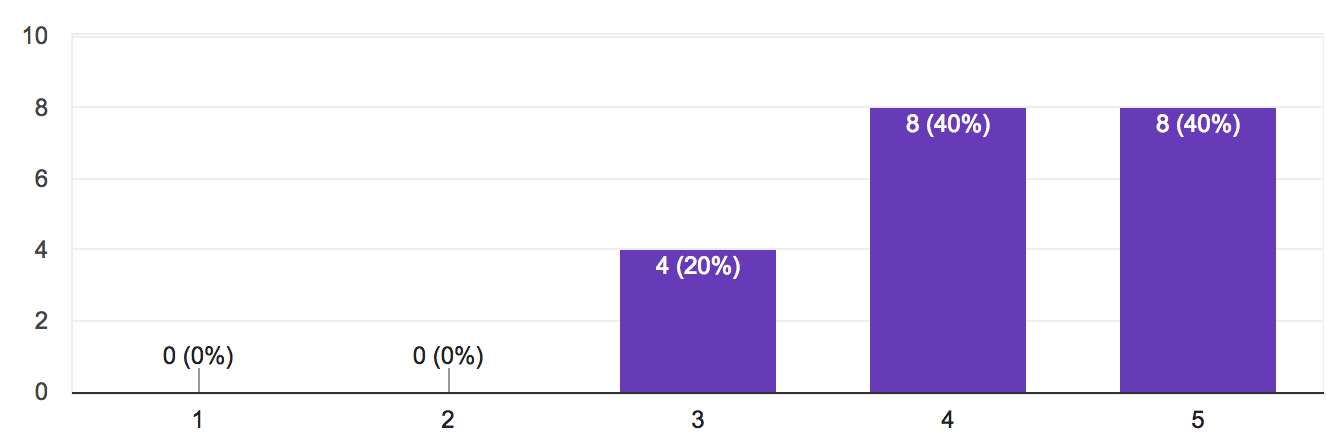
\includegraphics[width=0.8\columnwidth]{figures/opinions/reader_ease_of_use}
      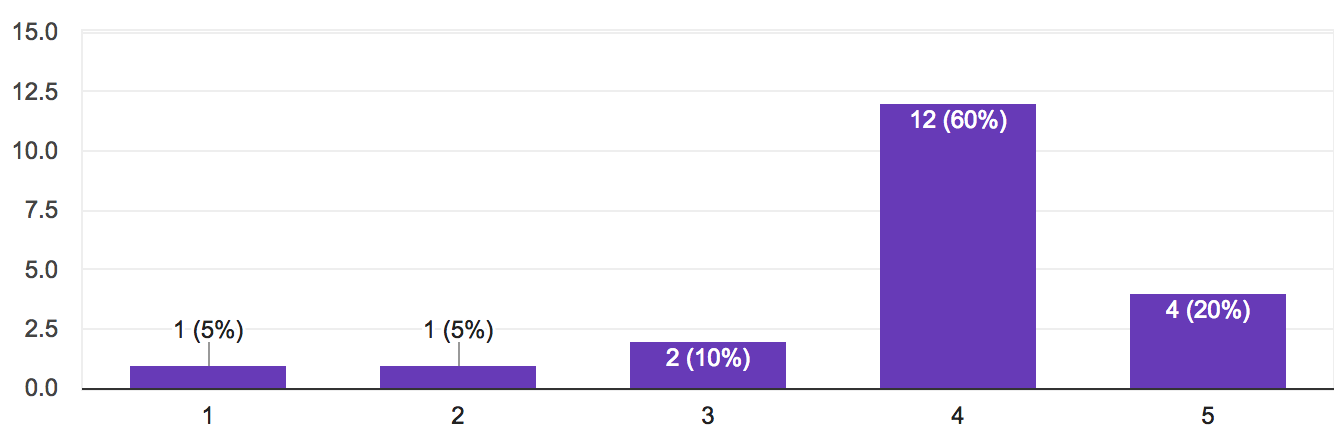
\includegraphics[width=0.8\columnwidth]{figures/opinions/reader_usefulness}
      \caption{Students assess ease of use and the usefulness of the reader}
      \label{fig:reader_use}
    \end{figure}

We asked the participants what would make their experience better. Many thought that the system was good the way it was, and a few others had some more specific answers (e.g. night reading mode, etc.). \footnote{The complete feedback is available in the GitHub repository of the paper.}. The most requiring requests were: 

\begin{itemize}
	\item Choice of Topics: 
		\squote{Order in different subjects like animals, politics, fashion...}, 
		\squote{Add a choice for different topics not only for the sources}, 
		\squote{Better display of the articles and tags such as 'gaming' or 'news'}, etc.
	\item More freedom for chosing materials: 
		\squote{Would be nice to be able to add website to the list} and 
		\squote{A search engine}. 
\end{itemize}

When asked about what they dislike about the Reader, the majority of feedback was related to translations: two people complained about them being in English (\squote{The translations are always in English}), five people complained about the translation quality (e.g. \squote{Some weak translations}). The English translations are the reason for which one learner reported that they prefer the textbook: \squote{The translations are always in English. This is why I would grab a textbook first. I don't want to look up the (English to) Dutch translation.}

Figure \ref{fig:ex_rating} shows that when asked to provide their personal rating of the the quality of the exercises, the majority of the respondents expresses their appreciation. 

 \begin{figure}[h!]
    \centering
      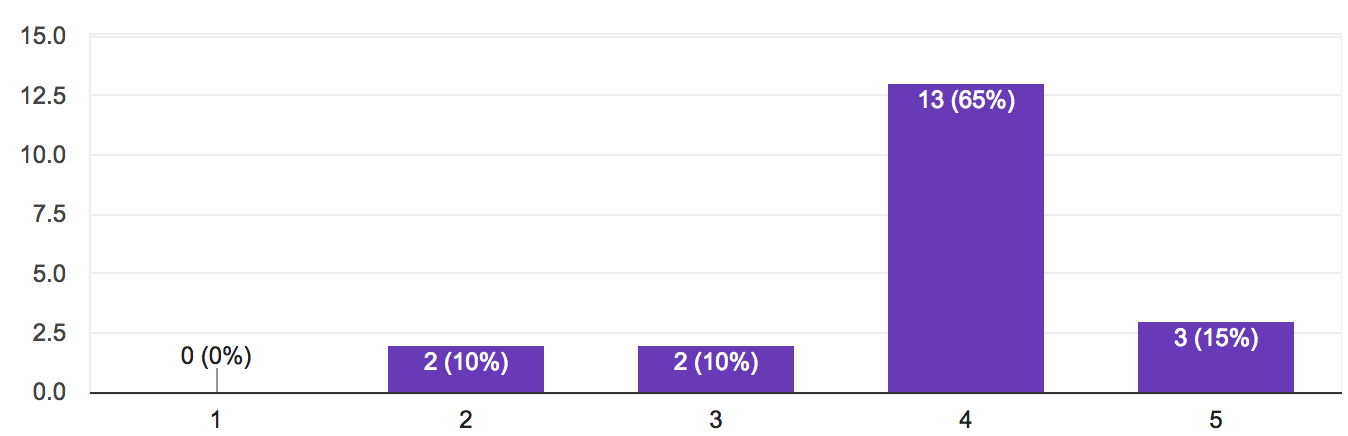
\includegraphics[width=0.8\columnwidth]{figures/opinions/exercises_rating}
      \caption{Students assessment  of the generated exercises}
      \label{fig:ex_rating}
    \end{figure}

When asked about what they dislike about exercises, many said literally ``nothing''. However, several also had concrete feedback: 
\begin{itemize}
	\item During exercises, translations are disabled, so if one does not understand a word from the context, they will have a difficulty.
		\squote{There aren't translations},
		\squote{Doesn't give the translations}
	\item Difficulty is not always appropriate: \squote{Some exercises are too easy}
	\item Contexts are always the same: \squote{I would like to see the words I practice in a different context}
\end{itemize}

Finally, we asked whether our learners would prefer our system to a textbook if offered the choice. We thus asked them what would they choose between the Zeeguu Reader (our system) and a textbook. We also gave them the possibility to answer something else with a free-form text field. Figure \ref{fig:preferred_reader} shows that the majority of the learners who answered our post-usage survey would prefer our system. However, some still prefer a textbook. 

 \begin{figure}[h!]
    \centering
      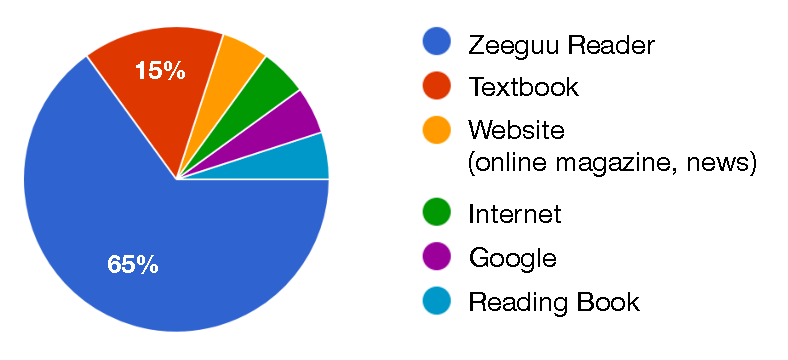
\includegraphics[width=1.05\columnwidth]{figures/opinions/reader_vs_textbook}
      \caption{Answers to the question: {\em ``If you wanted to read something in the language you study, what would you reach out for first?''}}
      \label{fig:preferred_reader}
    \end{figure}



\subsection{In-App Feedback}
Besides the analysis  based on the observed telemetry data, we also asked the students a series of questions by popping up questions while they were using the system. To do this, we used an online tool called HotJar. Among the questions was whether they preferred the reading platform and why. Some of the answers can be seen in the screenshot below. It becomes clear that the students appreciate the possibility of reading what is interesting for them.

    \begin{figure}[h!]
    \centering
      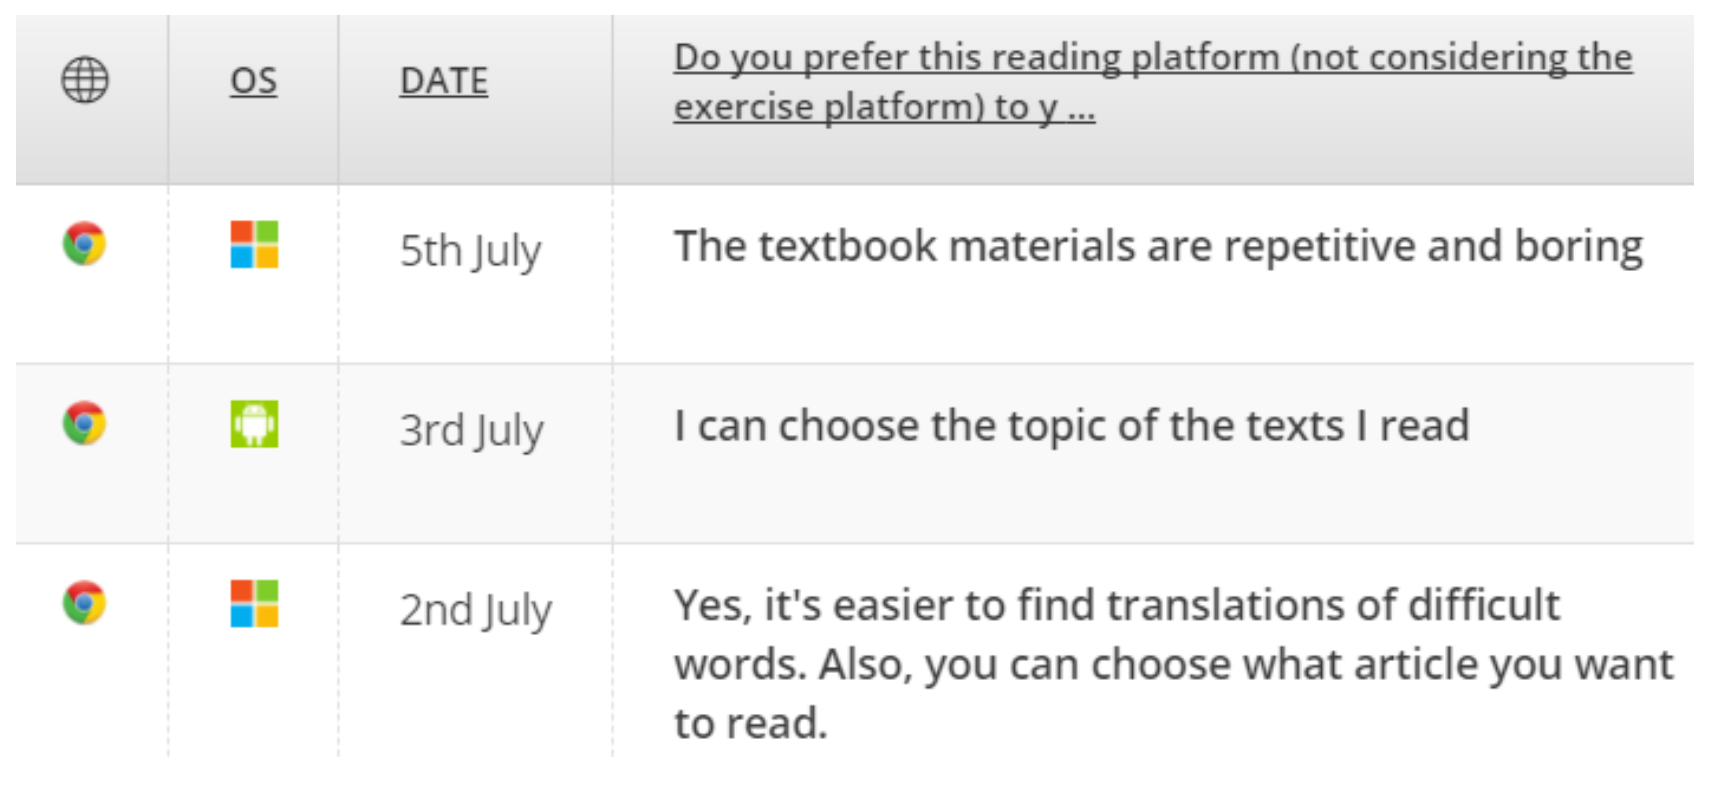
\includegraphics[width=\columnwidth]{figures/opinion_on_reading_platform}
      \caption{The students appreciate the freedom of choosing what to read}
    \end{figure}


\newpage
\subsection{Reports to the Teacher}
To triangulate the answers that they provided to us, we report here also what the students wrote in a separate evaluation of the tools they use in the class, which the teacher runs always at the end of the school year. Several of the answers are: 

\begin{description}
  \item {\em ``It works well but it were better if the translation would have been in Dutch. It is good that you can choose what to read.''}
  \item {\em ``Good for reading skills. Would have been best if it were in Dutch.''}
  \item {\em ``Your vocabulary is really moving forward, but then you have to do it more often than a few times. Overall a nice website, easy and fun subjects''}
\end{description}

There main message in the feedback is that learners appreciate the freedom of choosing materials to read that are personally interesting for them. The second, implied observation is that they appreciate the translations, but they would want to have them in their native language. 

\subsection{The Evaluation of the Teacher}
The teacher of the class appreciated the system, and decided to introduce it in the entire new academic year with a larger group of students. However, not all the new classes are bilingual, we will have to explore the best approach for situations in which the L1 is not English but Dutch.

% The way forward is then, by providing better recommendations if possible, and by providing translations in their native languages.

% In the future we plan to investigate whether the system works well enough with Dutch.

%!TEX root=paper.tex

\section{Limitations of this Study}
\label{sec:limitations}
% We presented a system, and we showed that it has the potential to generate user involvement. However the study we performed is not sufficient to reach a strong conclusion about the impact of the system we present... 

The feedback from the users was overall positive, with many of them showing appreciation for the personalization aspects of the system. However, more studies would be welcome since there are multiple reasons for which these results might not extend to the broader population. The students might have been influenced by our enthusiastic presentation of the system at the beginning of the testing month. Also, the number of students who answered our survey was limited: only \surveyrespondents students which represents less than 50\% of the participants who actually used the system.

We showed that the users are using the system extensively. However, this might be because the students were encouraged to use the system as part of their assignment in the class. We showed that the majority of the students used the system constantly throughout the one month period. If they only used it only for the final grade, we would have expected a more focused cramming at the end of the period (which we actually saw with a few of the students, but not with the majority). 

The students we worked with are not necessarily representative for the Dutch highschool student population since they are bilingual. Even in this case, during the feedback multiple of them opined that they would prefer to use the system in their native Dutch as opposed to English.

% We observed that students prefer to interact with different texts...  

The algorithms for scheduling vocabulary exercises are the state of the art in spaced repetition. However, we did not have a control group to see whether this approach works better than others. Moreover, note that other approaches for using spaced repetition already exist; what is unique in our approach is that the students learn based on personalized exercises generated based on the context of their past readings.




\newpage
\section{Challenges}
\label{sec:challenges}

In this section we explore some of the challenges that we perceive need to be addressed by our system and similar ``personal textbook'' systems. We base our list of challenges on our observations and on the feedback that we received from our learners. The full list of recommendations from our users can be found in the GitHub repository online.

\subsection{Registering for ``topics'' instead of ``sources''}
Multiple learners asked for the possibility of registering to article topics rather than ``article sources''. A future system should consider this.

\subsection{Ensuring the appropriateness of articles}
The advantage of a textbook is the fact that the quality control of the texts in it is guaranteed by the editors. How are we going to ensure the quality of the texts that re to be found online? What we did was to limit the possible sources from where the students can read. Nevertheless, one of the students, wrote in the feedback form {\em ``I would like to avoid articles which have information about accidents with human casualties''}. One thing that we plan to investigate in the future is crowdsourcing and ``teachersourcing'' where learners and teachers (or more generally, trusted advanced learners) can provide feedback on existing materials. Crowdsourcing has been identified by Heffernan et al. as one of the driving technologies of the upcoming adaptive learning \cite{Heff16-crowdsourcing}. 

% \subsection{The selection of vocabulary to study}

% How do we automatically verify the ``learnability '' of an example in the context? It is a great responsibility automatically selecting a word to study. The situation where a user accepted a mistaken translation, and then the system ``teaches'' the learner that word would be disastruous. Currently we have a set of filters that try to avoid this, moreover, we also offer the learner the possibility of providing feedback in case he is not confident in a given translation. In the future, we consider using crowdsourcing to decrease even more the probability of wrong translations.
% \ml{alternate perspecitve: Do the learners choose the right translation? }% 	\item provide shorter sentences


\subsection{Scheduling vocabulary exercises}
We have implemented the vocabulary practice scheduler in such a way that it tries to optimize the times when the words are being repeated based on the state of the art in spaced repetition. However, we received multiple requests from the users who are asking for the possibility of rehearsing the words in a given text, once they are finished with its study, more in the vein of traditional textbooks. It might be that in the future it would be useful to allow the learners to influence the scheduling algorithms. 

% A few other types of improvement ideas that we have received from our beta-testers are: 
% \begin{itemize}
% 	\item be forgiving with misspellings, allow retry if the learner was close instead of considering it a mistake
% 	\item better provide hints than simply showing the answer
% \end{itemize}


\subsection{Evaluating the quality of examples}

It is indeed desirable to find good examples of practice exercises from past readings. Sometimes, the context in which the learner looks up a word is too long and sometimes it is too short. How estimate the quality of an exercise? One measure that we are considering is: ensuring that all the words in the context are simpler than the tested word. 

% For beginners, this is still not an option. So we can only do this for students who are already quite advanced. \todo{We should see whether there's a difference between the ones that were A2 vs. B1}

\subsection{Estimating article difficulty in a personal way}
The way we did difficulty ranking was sub-optimal. Most of the difficulties were very close to each other in value, between 1 and 4 and they were generic instead of being personalized. We think that as a result, the difficulty estimations that the system presented were too abstract for the readers. And as a result, one of the readers reported that he disliked about the Reader the fact that \squote{My level of the language is quite low for now, so I clicked to get a translation very often. Too often.} 

A more advanced strategy is needed, one that is less abstract, and personalized for the individual learner. One approach would be to estimate the number of words that are likely to be unknown in an article for a particular learner. A complementary information about the article could be the number of words that we know are being learned at the moment which are to be found in that article. In this way, a learner can choose a text that also gives them the chance to re{\"e}ncounter words being learned. 

\subsection{The teacher perspective}
The system we presented here has a (limited) teacher dashboard for those users who have a teacher. The dashboard currently shows a chronological log of the words that the student has looked up in the context. However, the system could present more advanced analytics that could enhance the teacher's understanding of the class. This is something that is a clear opportunity when moving to a digital textbook. 

\subsection{Investigating more possible classroom workflows}
The system was initially designed for self study. However, when invited to test it in a formal classroom we were happy to oblige. We plan to work more with teachers to better understand how to combine the individuality of the system with the shared experience of the learners in a classroom. Indeed, new workflows and classroom activities must be discovered.


\section{Conclusion and Future Work}
We have presented here a system that we aimed to be a minimal viable product for a personalized language textbook. We report on using the system with high school students for about one month. We observe that overall the students make use of the personalization features, and when asked about it they appreciate them. The teacher of the class also appreciated the system, and decided to introduce it in the new academic year with a larger group of students. 


\section{Availability of System, Code and Data}

% \subsection{Software}
The system described in this paper is deployed and available online. If the readers of this article want to test it they can use the {\em CHI2018} invite code while following the  ``Become a Betatester'' link at \url{https://zeeguu.unibe.ch/}.

The source code is open under a MIT license and available online at \url{https://github.com/zeeguu-ecosystem}. To replicate this paper with another population, one can deploy their own version.

% \subsection{Data}
The anonymized telemetry data, representing the interactions of more than \students learners with the system for one month, is available as a MySQL database dump on GitHub at the following link: \url{https://github.com/zeeguu-ecosystem/CHI17-Paper}. The same link holds the full questionnaire data used in this paper. That data is also anonymized. 

We hope that the availability of the system, code, and the open data that we publish here will make it easy for other researchers to investigate problems related to personalization in foreign language reading.




% Balancing columns in a ref list is a bit of a pain because you
% either use a hack like flushend or balance, or manually insert
% a column break.  http://www.tex.ac.uk/cgi-bin/texfaq2html?label=balance
% multicols doesn't work because we're already in two-column mode,
% and flushend isn't awesome, so I choose balance.  See this
% for more info: http://cs.brown.edu/system/software/latex/doc/balance.pdf
%
% Note that in a perfect world balance wants to be in the first
% column of the last page.
%
% If balance doesn't work for you, you can remove that and
% hard-code a column break into the bbl file right before you
% submit:
%
% http://stackoverflow.com/questions/2149854/how-to-manually-equalize-columns-
% in-an-ieee-paper-if-using-bibtex
%
% Or, just remove \balance and give up on balancing the last page.
%

\newpage

\balance{}

% BALANCE COLUMNS
\balance{}


% REFERENCES FORMAT
% References must be the same font size as other body text.
\bibliographystyle{SIGCHI-Reference-Format}
\bibliography{mir-biblio/aslan}

\end{document}

%%% Local Variables:
%%% mode: latex
%%% TeX-master: t
%%% End:
